% ================================================================== PART IV
\part{Results and what they mean}

\chapter{Reconstruction results}
All numbers are means over 10 noise seeds from \code{results/*.csv}. The baseline is $n=64$, $W=h$, $\sigma=1\,\%$, $\Delta t=0.05$, Poisson with all-Neumann edges and the zero-mean constraint, Eulerian $D\uu/Dt$.

\section{Verification: grid convergence on clean data}
First the code must be shown correct, with no noise and no window averaging (exact point samples).
\begin{figure}[H]\centering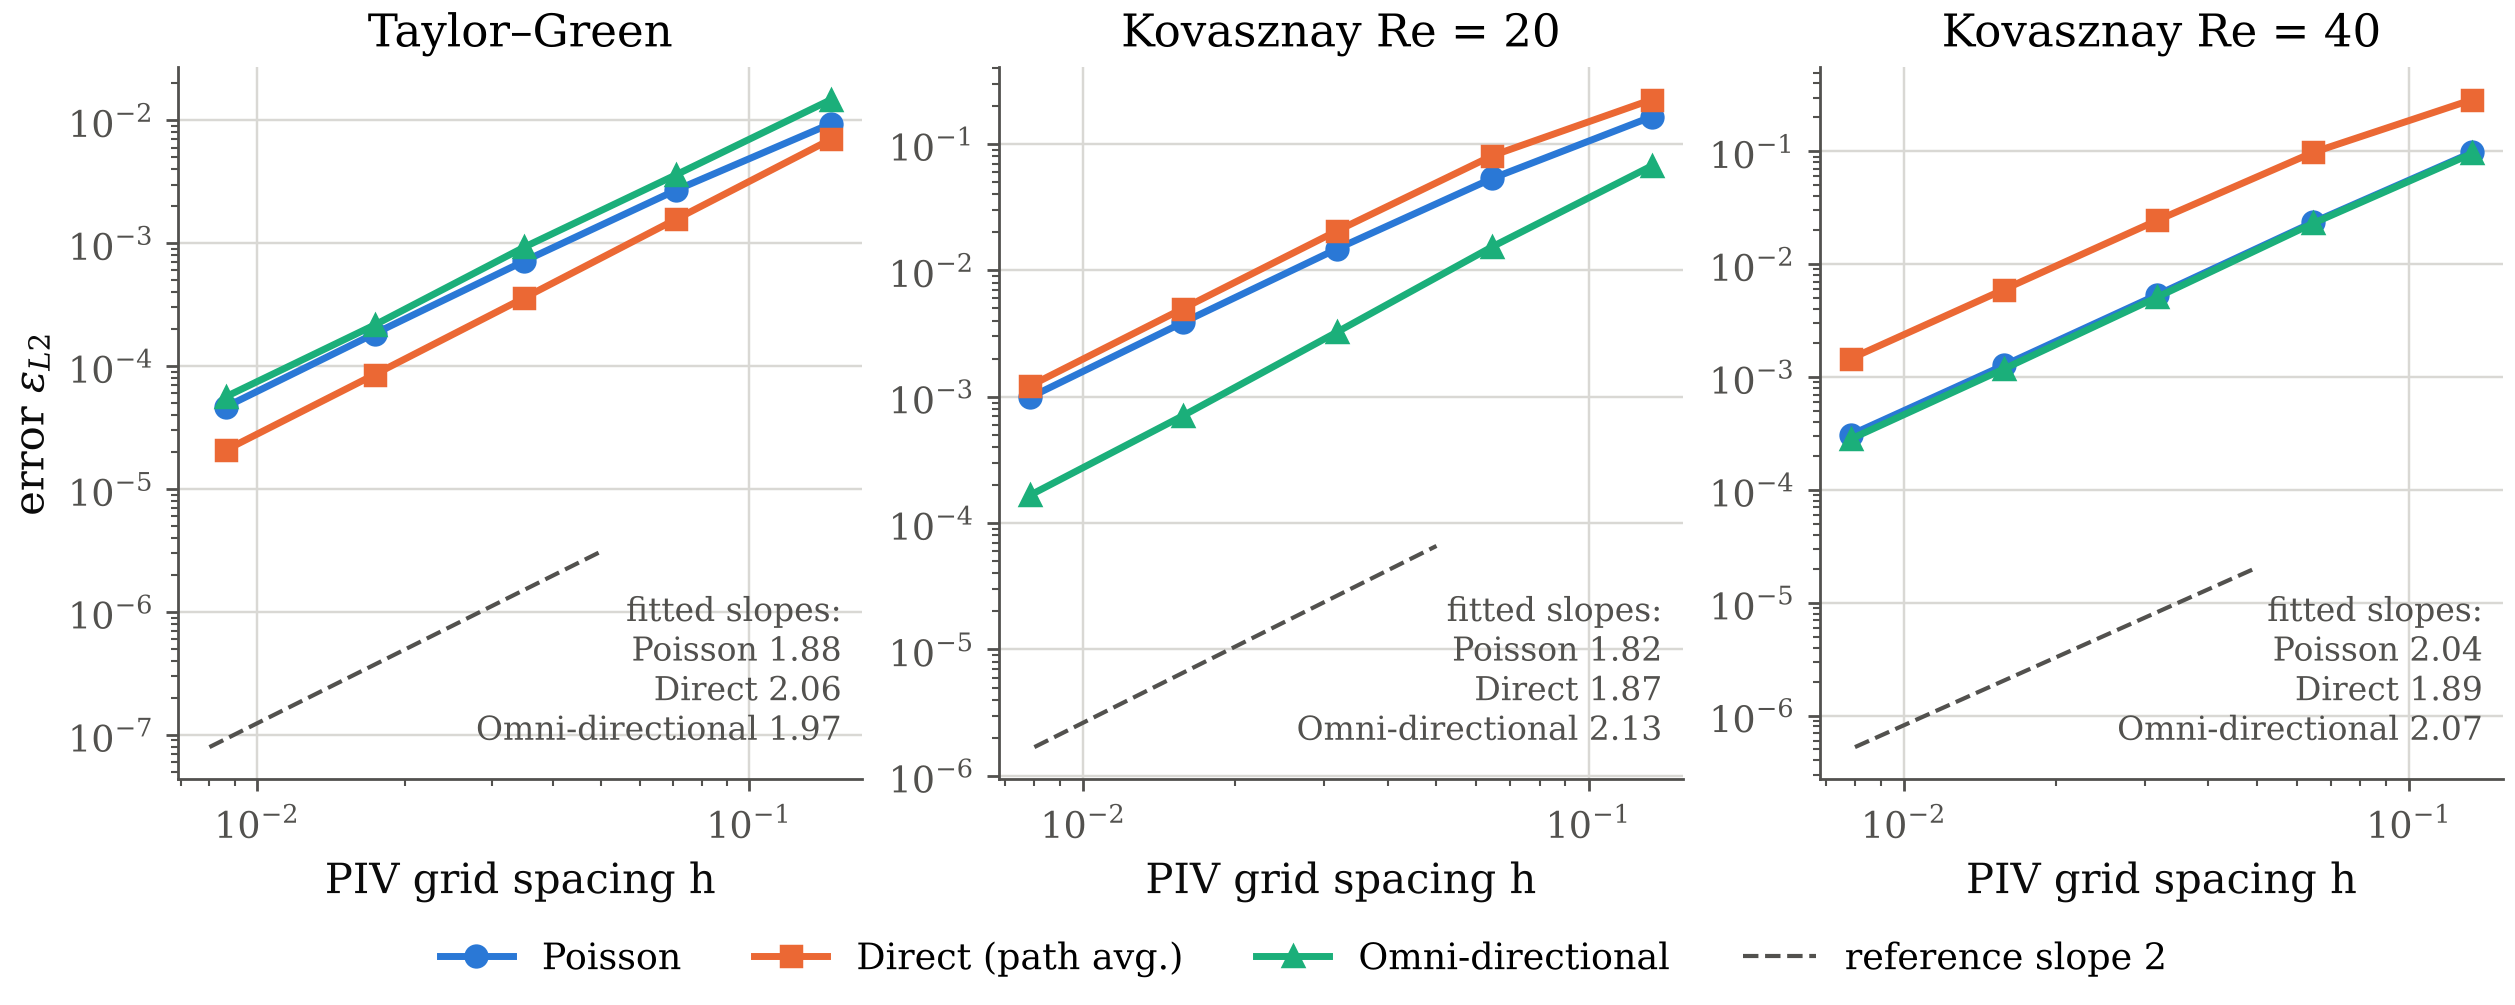
\includegraphics[width=\linewidth]{img/f_conv_clean.png}
\caption{Error vs PIV spacing on clean data for the three test flows and three methods; dashed line: slope 2.}\end{figure}

\begin{table}[H]\centering\small
\begin{tabular}{@{}lccc@{}}\toprule
Fitted slope of $\eps_{L2}$ vs $h$ ($16^2$--$256^2$) & Poisson & Direct & Omni\\\midrule
Taylor--Green & 1.88 & 2.06 & 1.97\\
Kovasznay Re = 20 & 1.82 & 1.87 & 2.13\\
Kovasznay Re = 40 & 2.04 & 1.89 & 2.07\\\bottomrule
\end{tabular}\end{table}

\textbf{What it shows.} All three methods are second-order accurate on all three flows, as the $O(h^2)$ stencils and trapezoidal rule predict. Between the two finest grids the local Poisson slopes are 1.96--2.03; fits over all grids are slightly lower because the coarsest grids are pre-asymptotic. The finest-grid errors are tiny ($4.7\times10^{-5}$ for Poisson on Taylor--Green at $256^2$). Kovasznay errors are larger at a given $h$ because its pressure varies steeply near the inflow edge ($e^{2\lambda x}$). The code is verified before any noise is added.

\section{Noise vs resolution: an optimum spacing}
\begin{figure}[H]\centering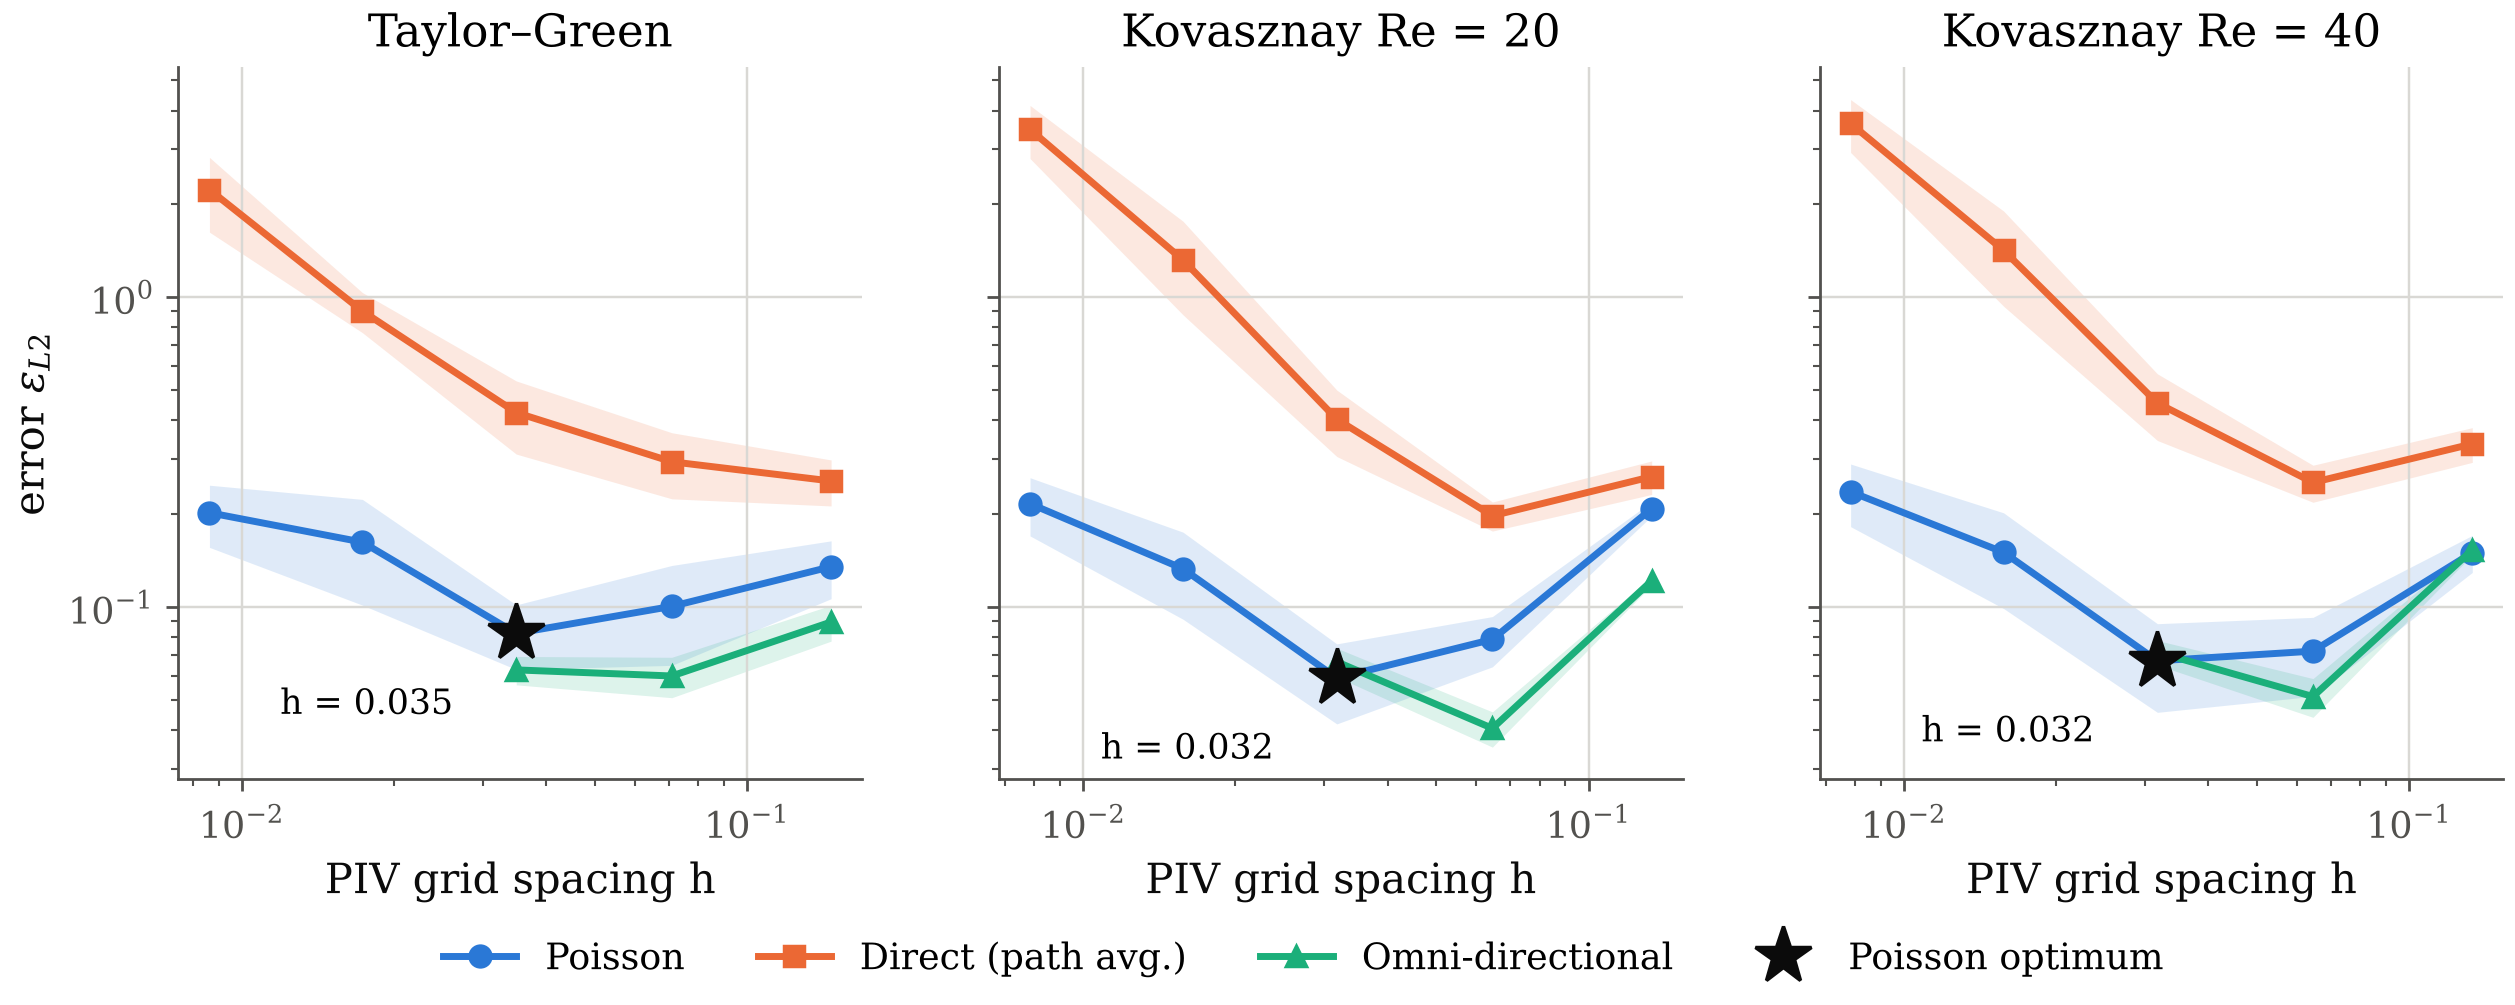
\includegraphics[width=\linewidth]{img/f_conv_noisy.png}
\caption{Error vs spacing with $\sigma=1\,\%$, $W=h$ (mean $\pm$ std of 10 seeds). Stars: the Poisson optimum.}\end{figure}

\begin{table}[H]\centering\small
\begin{tabular}{@{}rrccc@{}}\toprule
$n$ & $h$ (TG) & Taylor--Green & Kovasznay 20 & Kovasznay 40\\\midrule
16 & 0.147 & 0.135 & 0.208 & 0.150\\
32 & 0.071 & 0.101 & 0.079 & 0.072\\
\textbf{64} & \textbf{0.035} & \textbf{0.082} & \textbf{0.059} & \textbf{0.067}\\
128 & 0.017 & 0.162 & 0.133 & 0.150\\
256 & 0.009 & 0.202 & 0.216 & 0.236\\\bottomrule
\end{tabular}
\caption{Poisson $\eps_{L2}$ with 1\,\% noise. The minimum is at $n=64$ for all three flows.}\end{table}

\textbf{What it shows and why.} With noise, refining the grid stops helping: the Poisson error is lowest at $h\approx0.032$--$0.035$ ($n=64$) for all three flows and rises again on finer grids. This is the trade-off of Eq.~\eqref{eq:noiseG}. Truncation error falls as $h^2$, but noise is amplified as $\sigma/h$ by the convective term and as $\mu\sigma/h^2$ by the viscous term. At $h=0.035$ the viscous noise is already comparable to the convective noise, and it grows fastest.

\textbf{Direct integration only gets worse} as the grid is refined (Taylor--Green 0.26 $\to$ 2.2): a path crosses $\sim1/h$ noisy steps and its error grows like a random walk. On Kovasznay its optimum is at the coarser $h\approx0.065$.

\begin{keyidea}[Practical consequence]
For noisy PIV data there is a best vector spacing. Asking for the finest possible PIV grid can make the pressure \emph{worse}. The optimum moves to coarser grids as the noise level rises.
\end{keyidea}

\section{Noise sensitivity and choice of method}
\begin{figure}[H]\centering
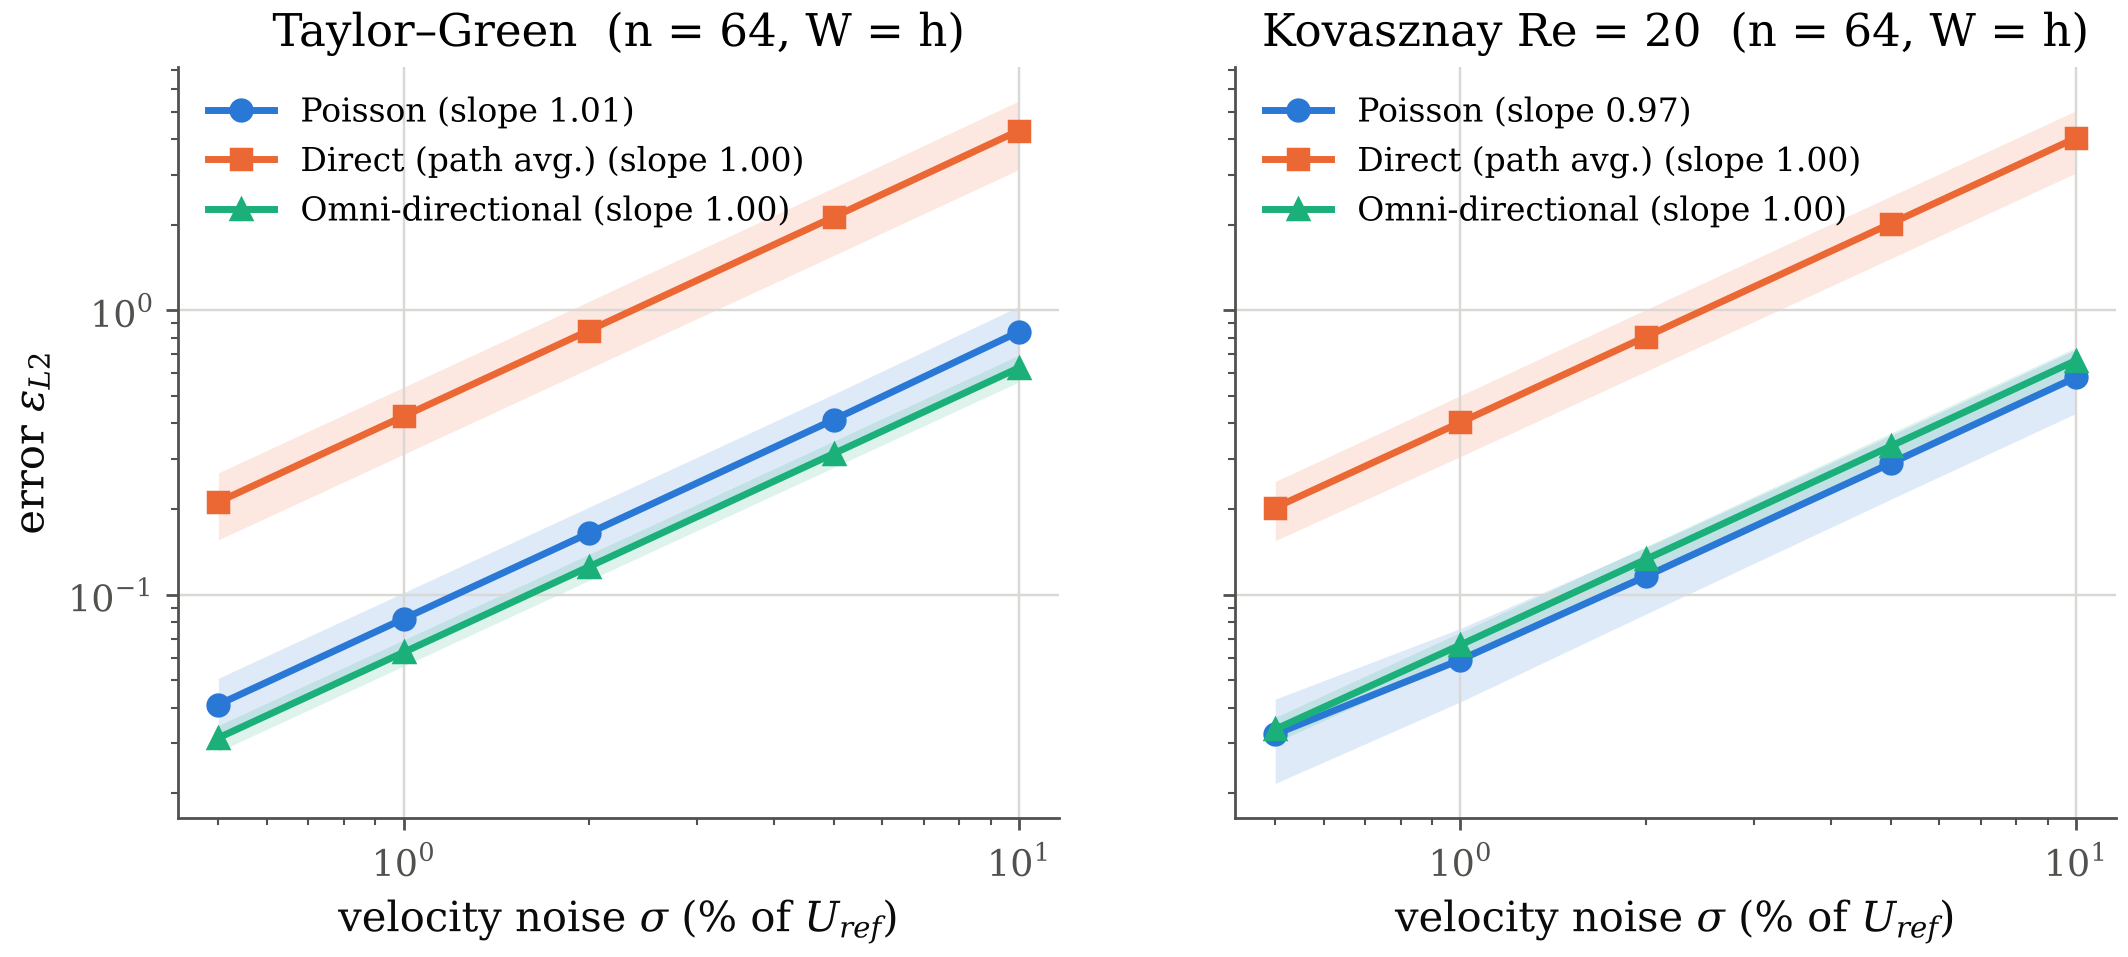
\includegraphics[width=0.85\linewidth]{img/f_noise.png}
\caption{Error vs noise level ($n=64$, $W=h$); the slopes in the legend are log--log fits.}\end{figure}
\begin{figure}[H]\centering
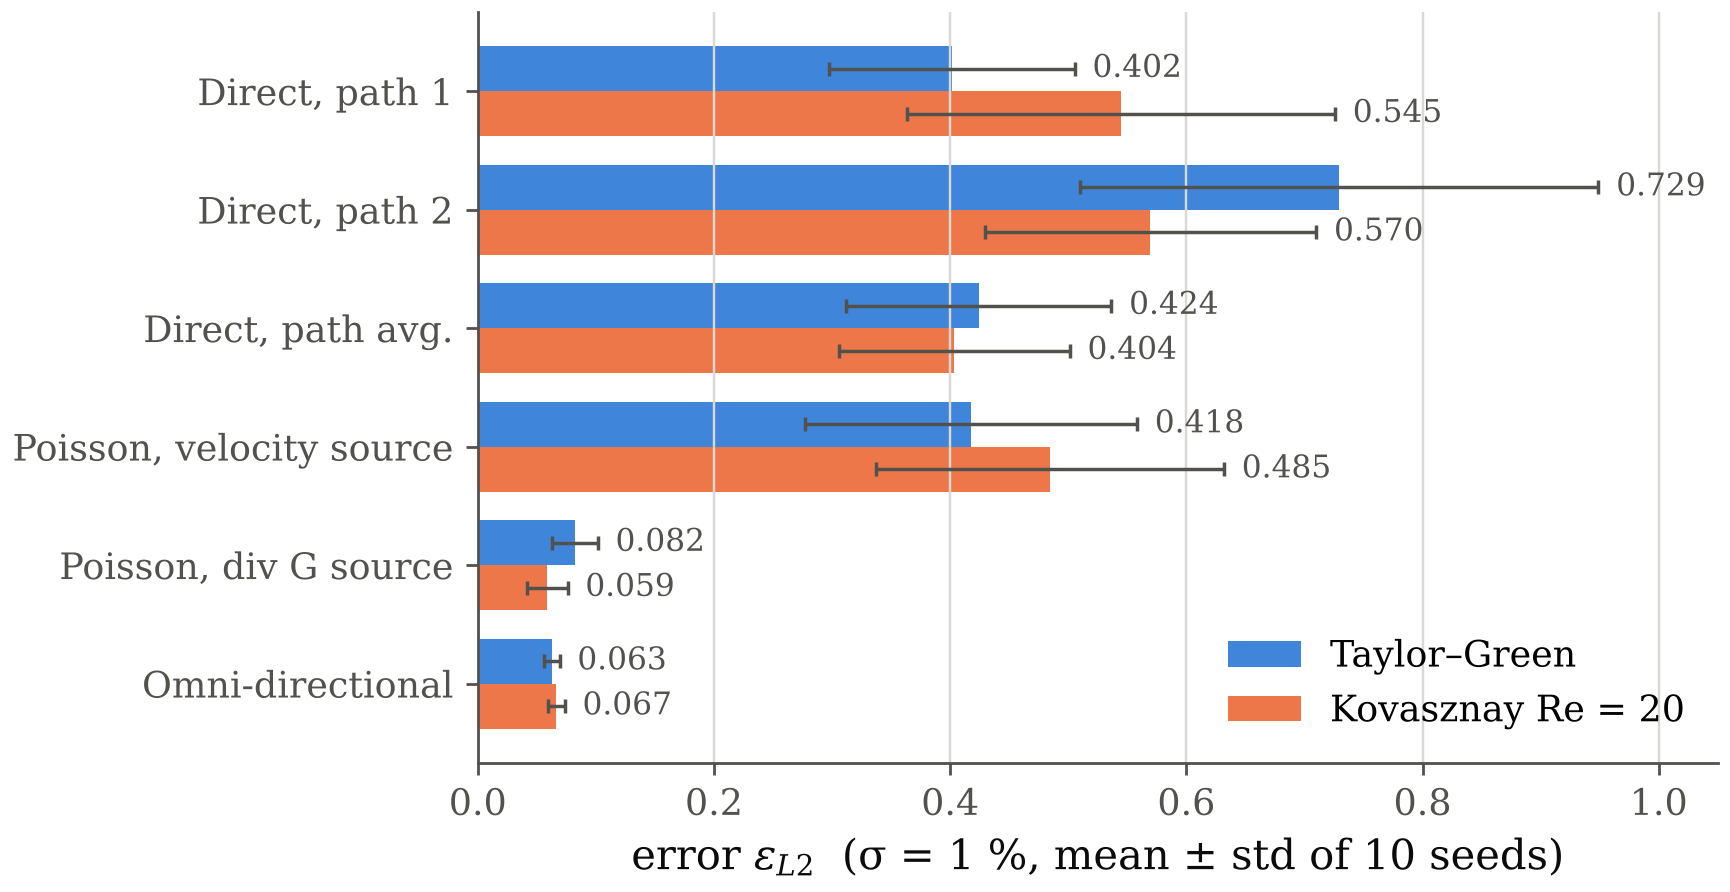
\includegraphics[width=0.62\linewidth]{img/f_method_bar.png}
\caption{All integration variants at $\sigma=1\,\%$ (mean $\pm$ std of 10 seeds).}\end{figure}

\begin{table}[H]\centering\small
\begin{tabular}{@{}lccccc@{}}\toprule
 & \multicolumn{2}{c}{$\eps_{L2}$ at $\sigma=1\,\%$} & \multicolumn{2}{c}{log--log slope vs $\sigma$} & Time per\\
Method & TG & Kov 20 & TG & Kov 20 & reconstruction\\\midrule
Direct (path avg.) & 0.424 & 0.404 & 1.00 & 1.00 & 0.3 ms\\
Poisson ($\nabla\cdot\G$ source) & 0.082 & 0.059 & 1.01 & 0.97 & 15 ms\\
Omni-directional & 0.063 & 0.067 & 1.00 & 1.00 & 0.41 s\\
Poisson (velocity source) & 0.418 & 0.485 & -- & -- & 15 ms\\\bottomrule
\end{tabular}\end{table}

\begin{enumerate}
\item \textbf{Error grows linearly with noise} (log--log slopes 0.97--1.01). The whole reconstruction is a linear operation on the velocity error (apart from the small quadratic convective term), so doubling the noise doubles the error.
\item \textbf{Direct integration is 5--7$\times$ worse.} A single path carries every error along it; Poisson (elliptic: every point sees the whole domain) and omni (average of 32 directions) average errors out.
\item \textbf{Omni and Poisson are equally accurate} (each wins one flow) but omni is about 27$\times$ slower. Poisson is the practical choice.
\item \textbf{Path 1 and path 2 differ} (Taylor--Green 0.40 vs 0.73). This is not a bug: mirroring the data ($x\leftrightarrow y$) swaps the two errors exactly. Noise in the convective and viscous terms comes from the same snapshot, so the terms are correlated; whether they add or cancel along a path depends on the flow direction relative to the path.
\item \textbf{The velocity-source Poisson form is 5--8$\times$ worse with noise.} Its interior source multiplies noisy derivatives, while its boundary data still come from $\G$, so source and boundary data no longer come from one vector field. The least-squares structure of Section~3.3.2 is lost. (With noise-free boundary data it was actually better: its weakness is the mismatch, not the identity.)
\end{enumerate}

\begin{figure}[H]\centering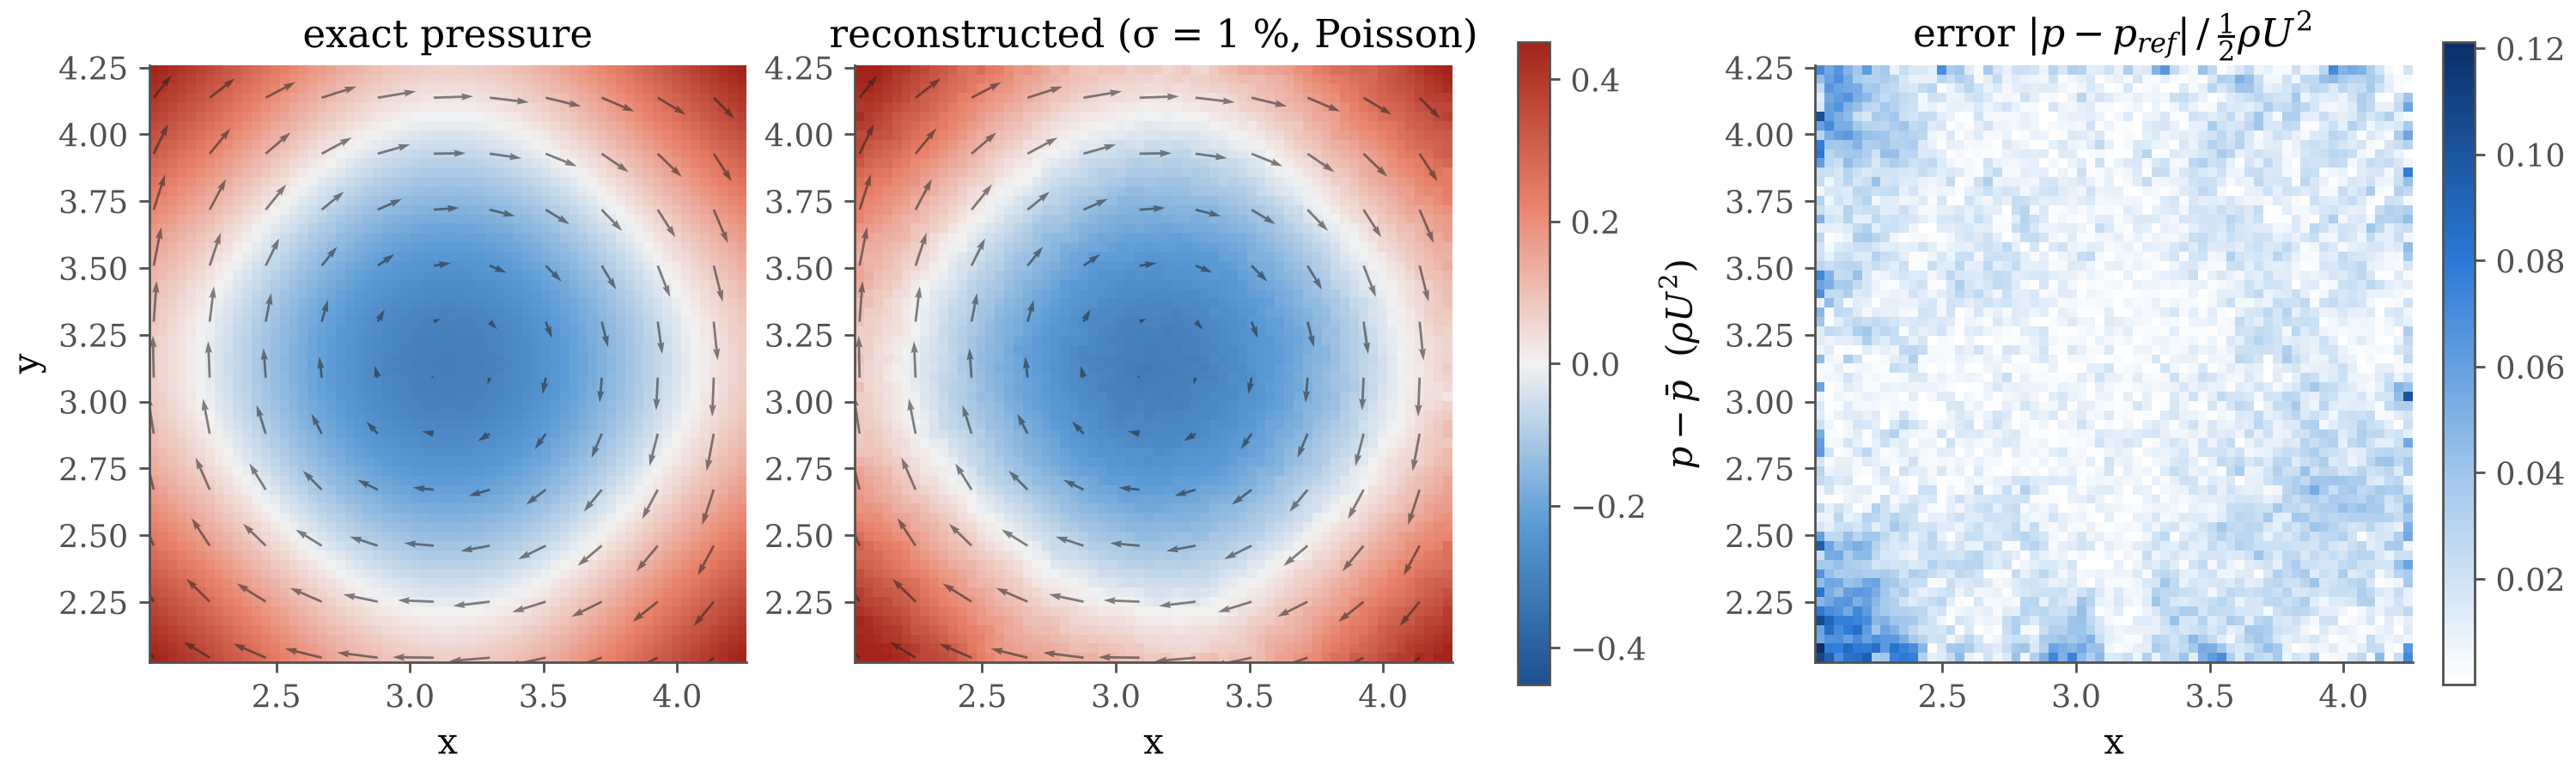
\includegraphics[width=\linewidth]{img/f_fields_tg.png}
\caption{Taylor--Green core window: exact pressure, reconstruction from noisy PIV-like data ($\sigma=1\,\%$, Poisson, $\eps_{L2}=0.061$ for this seed), and the error map. The vortex is recovered; the error is mostly random scatter, largest at the edges.}\end{figure}

\section{Boundary conditions for the Poisson solver}
\begin{figure}[H]\centering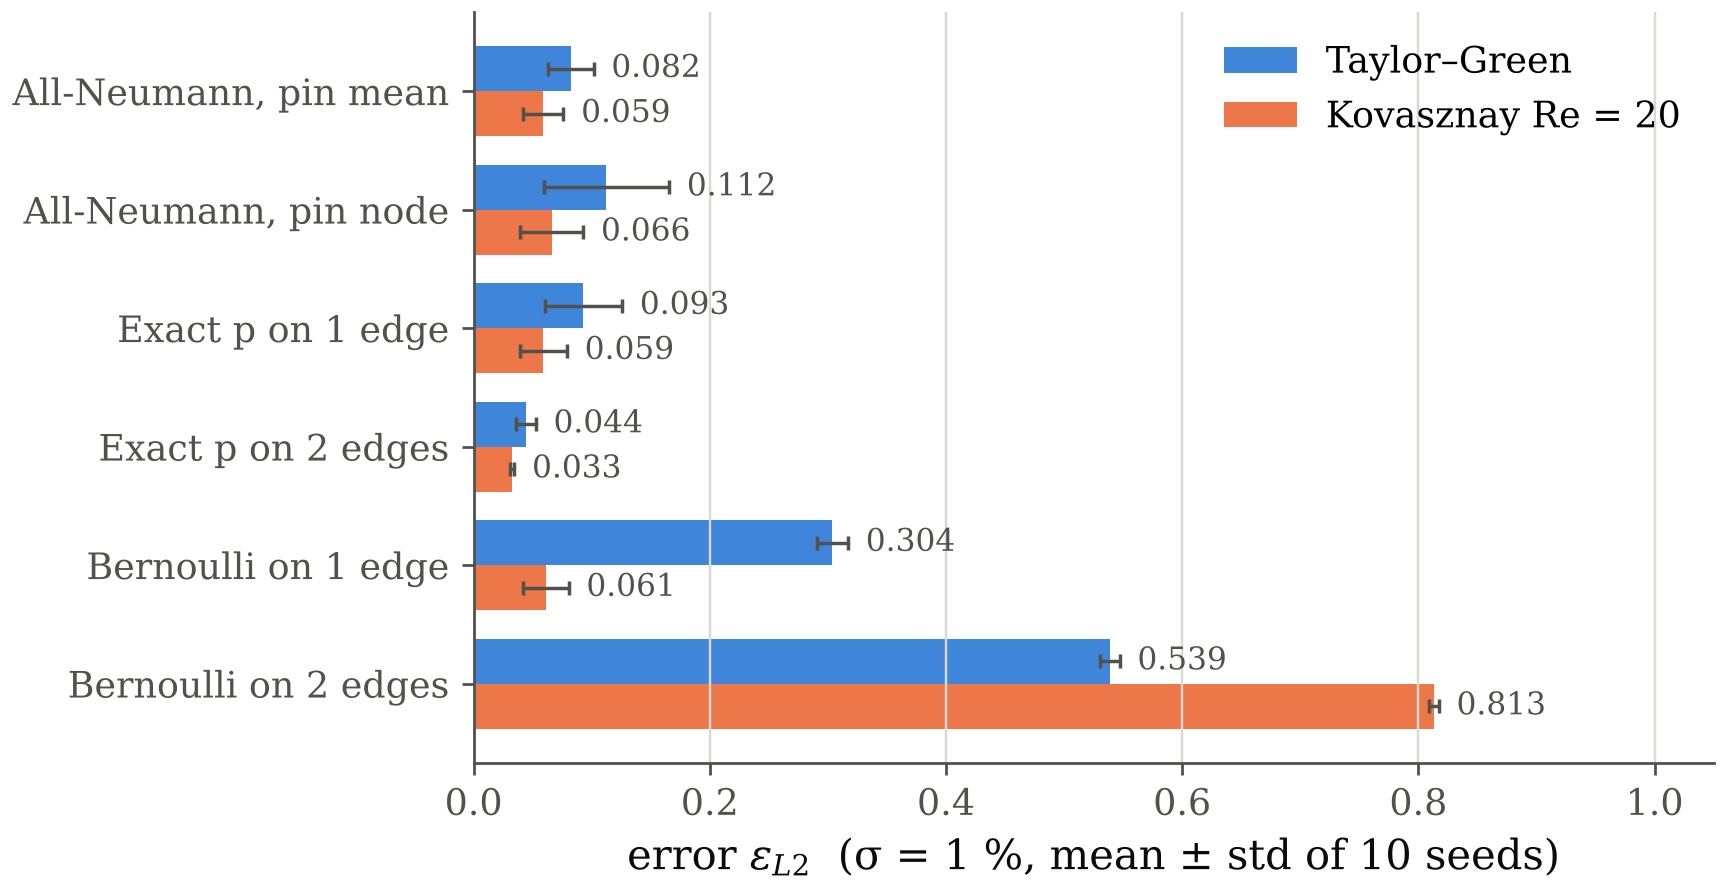
\includegraphics[width=0.62\linewidth]{img/f_bc_bar.png}
\caption{Poisson error for six boundary treatments at $\sigma=1\,\%$.}\end{figure}

\begin{table}[H]\centering\small
\begin{tabular}{@{}lcc@{}}\toprule
Boundary treatment & TG noisy $\eps_{L2}$ & Kov 20 noisy $\eps_{L2}$\\\midrule
All-Neumann, zero mean (baseline) & 0.082 & 0.059\\
All-Neumann, pin one node & 0.112 & 0.066\\
Exact $p$ on 1 edge & 0.093 & 0.059\\
\textbf{Exact $p$ on 2 opposite edges} & \textbf{0.044} & \textbf{0.033}\\
Bernoulli on 1 edge & 0.304 & 0.061\\
Bernoulli on 2 edges & 0.539 & 0.813\\\bottomrule
\end{tabular}\end{table}

\begin{enumerate}
\item \textbf{Known pressure on two opposite edges halves the error.} Neumann data $\n\cdot\G$ are themselves noisy derivatives, so their errors propagate inward; a Dirichlet edge anchors the solution. Two opposite edges bracket the domain. (The ``exact'' option is an oracle standing in for wall pressure taps.)
\item \textbf{One edge helps little or even hurts}: the Neumann-data error is anchored on one side only and accumulates across the domain.
\item \textbf{Pinning a node is worse than the zero-mean constraint}: it dumps the incompatibility at one point (Section~5.3).
\item \textbf{Bernoulli edges fail} (up to 0.81): $p+\tfrac12\rho|\uu|^2=$ const holds only in irrotational flow, and both flows are rotational everywhere. Use Bernoulli only at genuine free-stream edges.
\end{enumerate}

\section{Time step: Eulerian vs Lagrangian}
\begin{figure}[H]\centering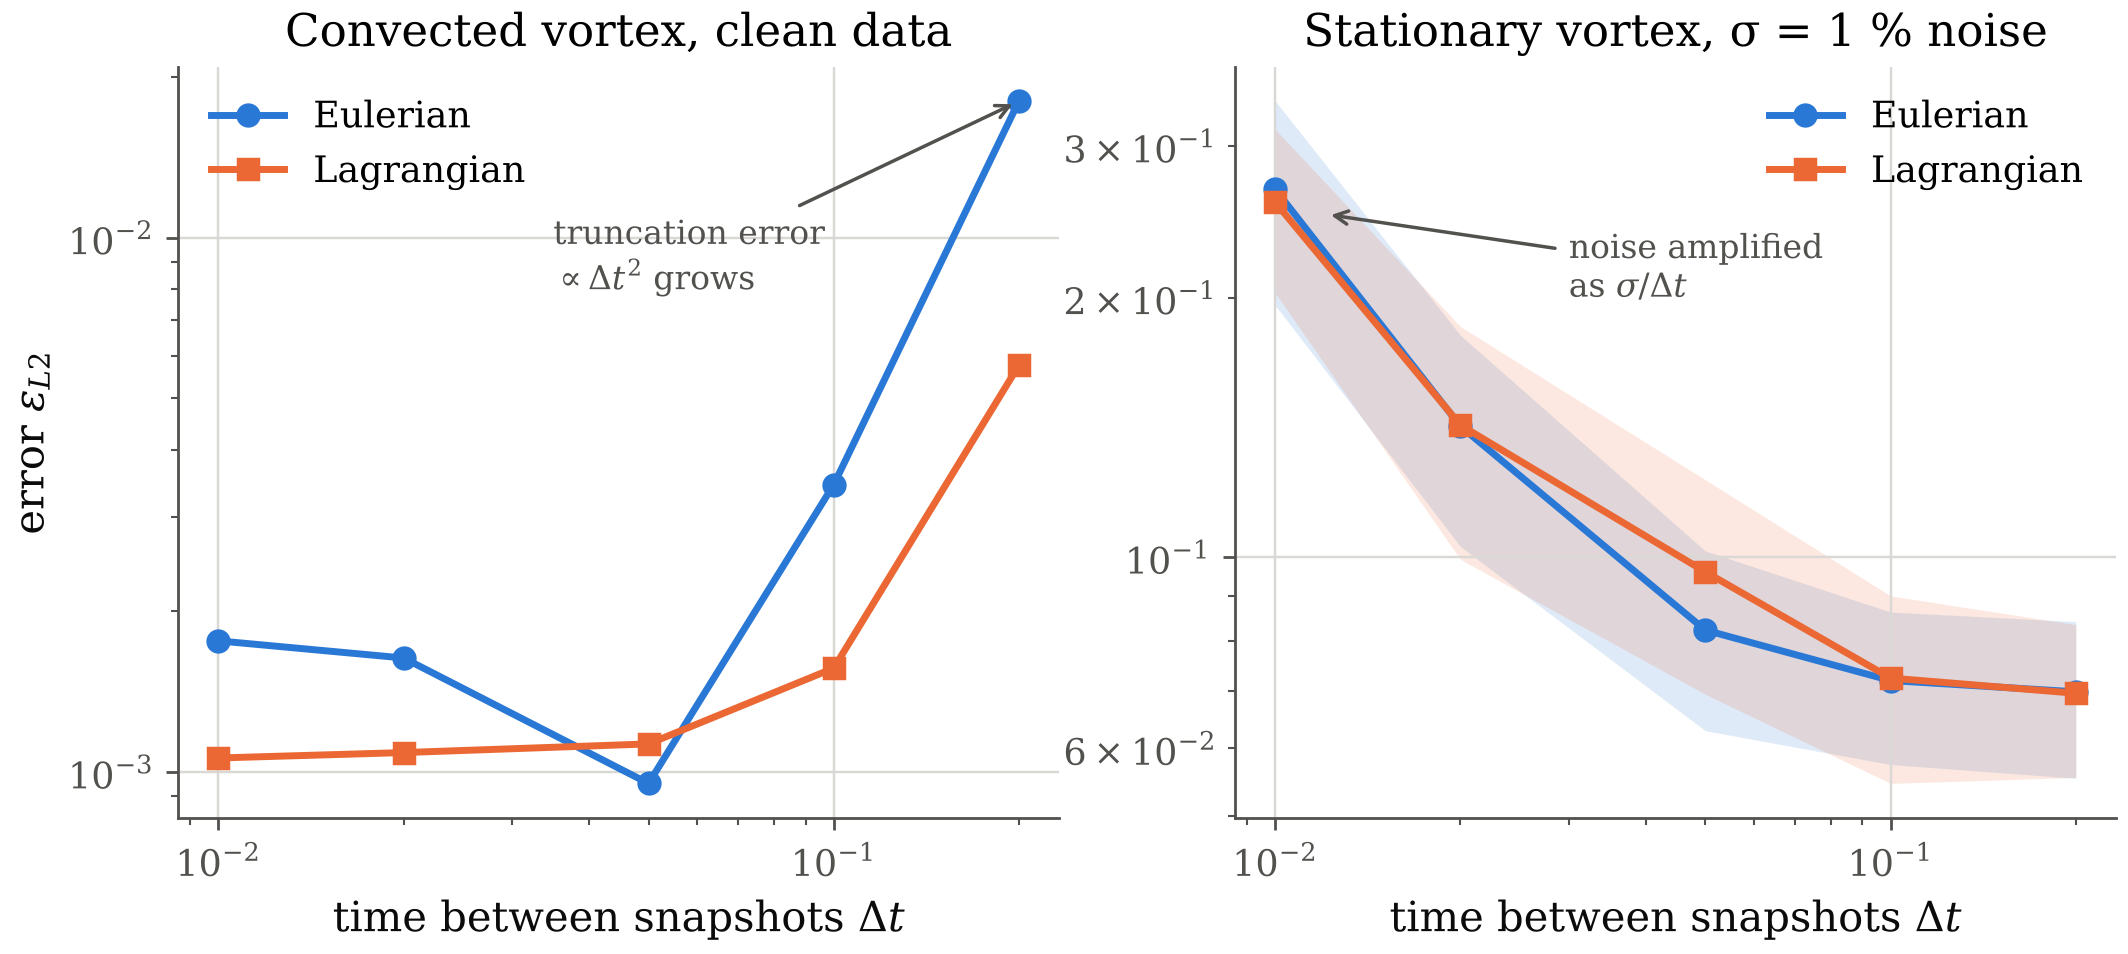
\includegraphics[width=0.85\linewidth]{img/f_dt.png}
\caption{Error vs time between snapshots. Left: convected vortex, clean data. Right: stationary vortex with 1\,\% noise.}\end{figure}

\begin{table}[H]\centering\small
\begin{tabular}{@{}rcccc@{}}\toprule
 & \multicolumn{2}{c}{Convected TG, clean} & \multicolumn{2}{c}{Stationary TG, $\sigma=1\,\%$}\\
$\Delta t$ & Eulerian & Lagrangian & Eulerian & Lagrangian\\\midrule
0.01 & $1.8\times10^{-3}$ & $1.1\times10^{-3}$ & 0.267 & 0.258\\
0.05 & $9.5\times10^{-4}$ & $1.1\times10^{-3}$ & 0.082 & 0.096\\
0.10 & $3.5\times10^{-3}$ & $1.6\times10^{-3}$ & 0.072 & 0.072\\
0.20 & $1.8\times10^{-2}$ & $5.8\times10^{-3}$ & 0.070 & 0.070\\\bottomrule
\end{tabular}\end{table}

\begin{enumerate}
\item \textbf{Convected vortex (clean):} the Eulerian error grows 10$\times$ from $\Delta t=0.01$ to 0.2, because at a fixed point the pattern sweeps past and $\partial\uu/\partial t$ changes quickly ($\propto c^3$). The Lagrangian scheme follows the particle; its error grows only with the vortex's own velocity ($\propto w^3$) and is 3$\times$ lower at $\Delta t=0.2$. This is exactly the $w/c$ argument of Section~3.2.
\item \textbf{Stationary vortex (clean):} the Eulerian error does not depend on $\Delta t$ (the flow barely changes at a point), while the Lagrangian error grows (to $4.2\times10^{-3}$ at $\Delta t=0.2$) because it traces curved particle paths with a straight step.
\item \textbf{Noisy data:} both schemes \emph{improve} with larger $\Delta t$ (0.27 $\to$ 0.07), because the noise in $\partial\uu/\partial t$ scales as $\sigma/\Delta t$ and dominates over this range. The best $\Delta t$ balances noise against truncation error, just like the best $h$.
\end{enumerate}

\section{Interrogation window and denoising}
\begin{figure}[H]\centering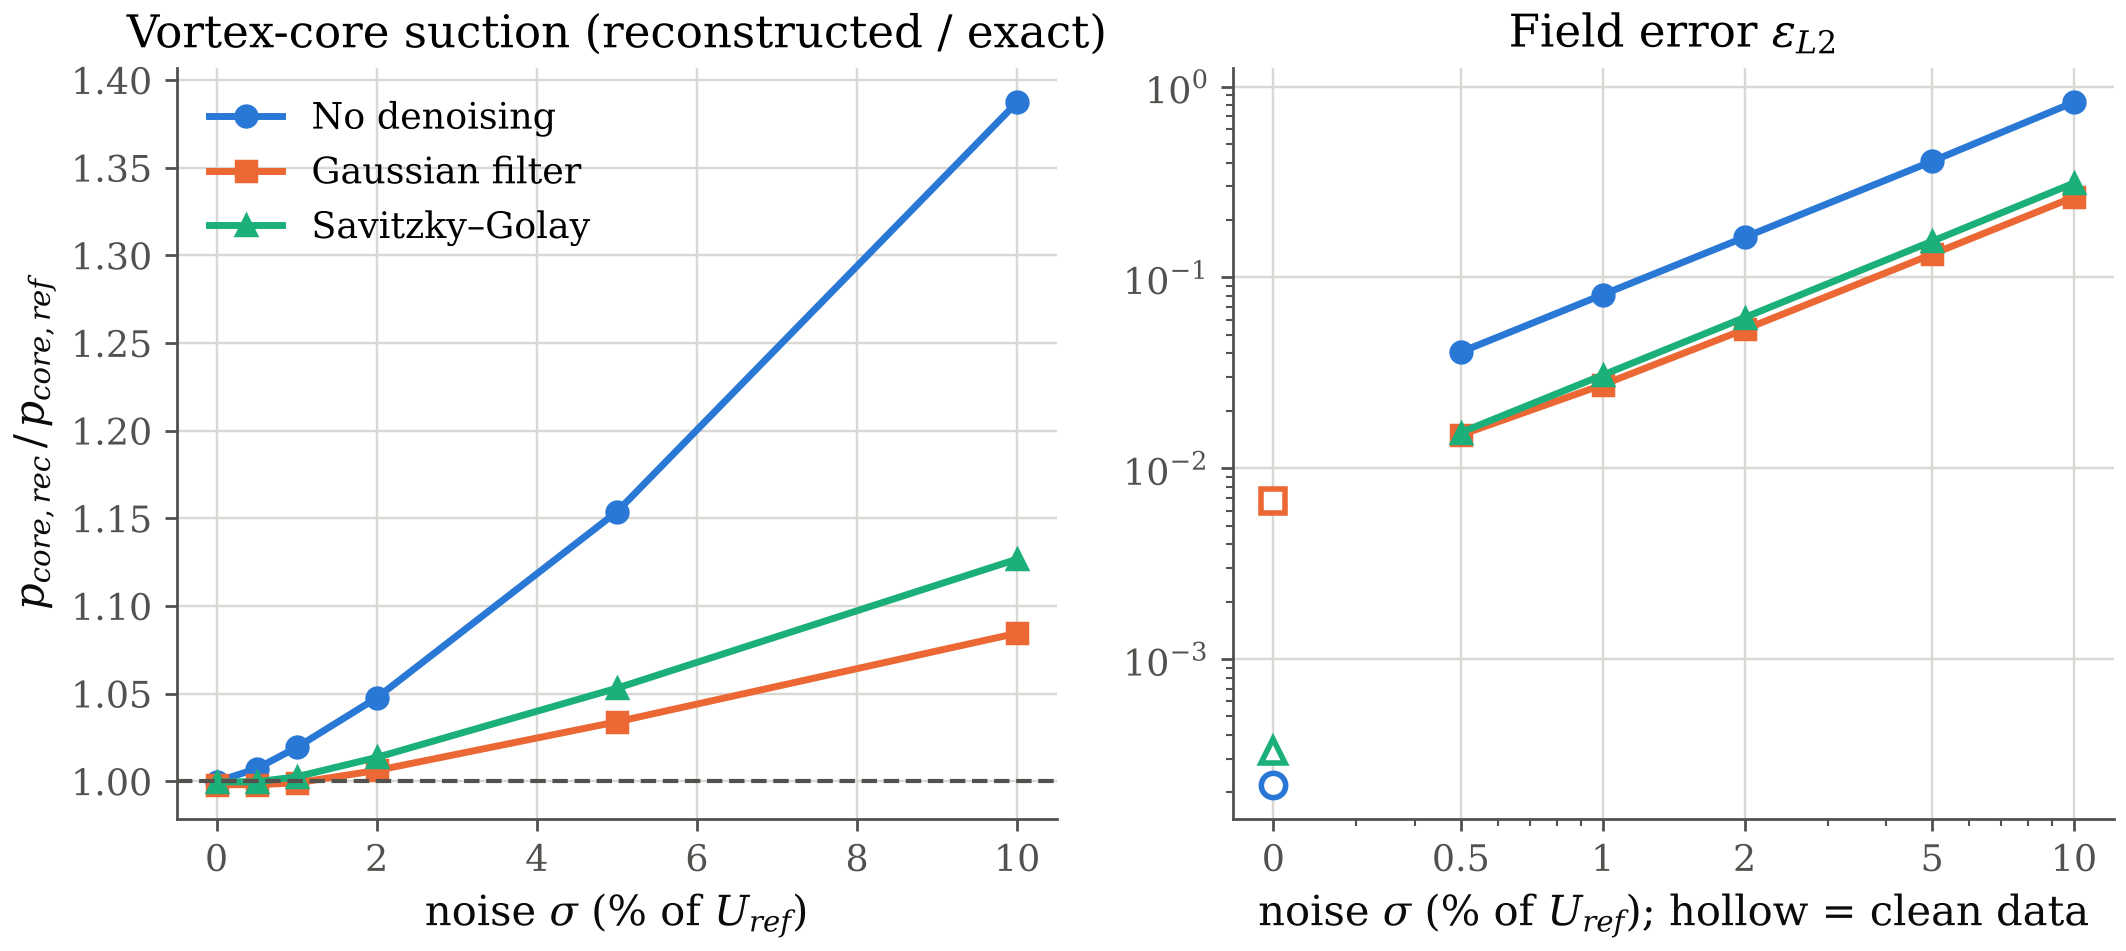
\includegraphics[width=0.85\linewidth]{img/f_denoise.png}
\caption{Taylor--Green core window. Left: reconstructed/exact vortex-core suction vs noise. Right: field error vs noise; hollow markers = clean data.}\end{figure}

\textbf{Window size $W$.} Averaging over the window smooths velocity. On the Taylor--Green core the suction drops only 0.3\,\% at $W=4h$, because the vortex (size $\sim\pi$) is much larger than the window ($4h\approx0.14$). On Kovasznay, with its sharp gradients near the inflow, $\eps_{L2}$ rises from 0.015 to 0.061 (clean). The effect grows with $W$ relative to the flow structure size, so it is expected to be much stronger for the cylinder-wake vortices.

\begin{table}[H]\centering\small
\begin{tabular}{@{}rccc@{}}\toprule
$\sigma$ (\%) & None & Gaussian & Savitzky--Golay\\\midrule
0 & 0.0002 & 0.0068 & 0.0003\\
0.5 & 0.041 & 0.015 & 0.015\\
1 & 0.081 & 0.027 & 0.031\\
2 & 0.162 & 0.053 & 0.062\\
5 & 0.406 & 0.132 & 0.155\\
10 & 0.828 & 0.264 & 0.312\\\bottomrule
\end{tabular}
\caption{Taylor--Green core window, $\eps_{L2}$ with and without denoising.}\end{table}

\begin{enumerate}
\item \textbf{Denoising cuts the noisy error about 3$\times$} at every noise level from 0.5\,\%.
\item \textbf{On clean data it hurts}: the Gaussian filter raises the error from 0.0002 to 0.007 because it also smooths the true signal. Savitzky--Golay barely changes clean data (it preserves quadratics), but on Kovasznay both filters help only above 0.5--1\,\%.
\item \textbf{Noise biases the core, not just scatters it.} Without denoising the core suction is \emph{over}-predicted, 1.39$\times$ at $\sigma=10\,\%$. The convective term multiplies noisy quantities, and products of zero-mean noise do not average to zero; also the minimum of a noisy field is biased low (a selection bias). Filtering reduces both.
\end{enumerate}

\begin{keyidea}[Smoothing trades noise for bias]
Window averaging, denoising and larger $\Delta t$ all reduce random error and add systematic error. The best setting depends on the noise level: none at $\sigma\approx0$, moderate above about 0.5\,\%.
\end{keyidea}

% ------------------------------------------------------------------
\chapter{Solver and convergence results}

\section{Residual histories}
\begin{figure}[H]\centering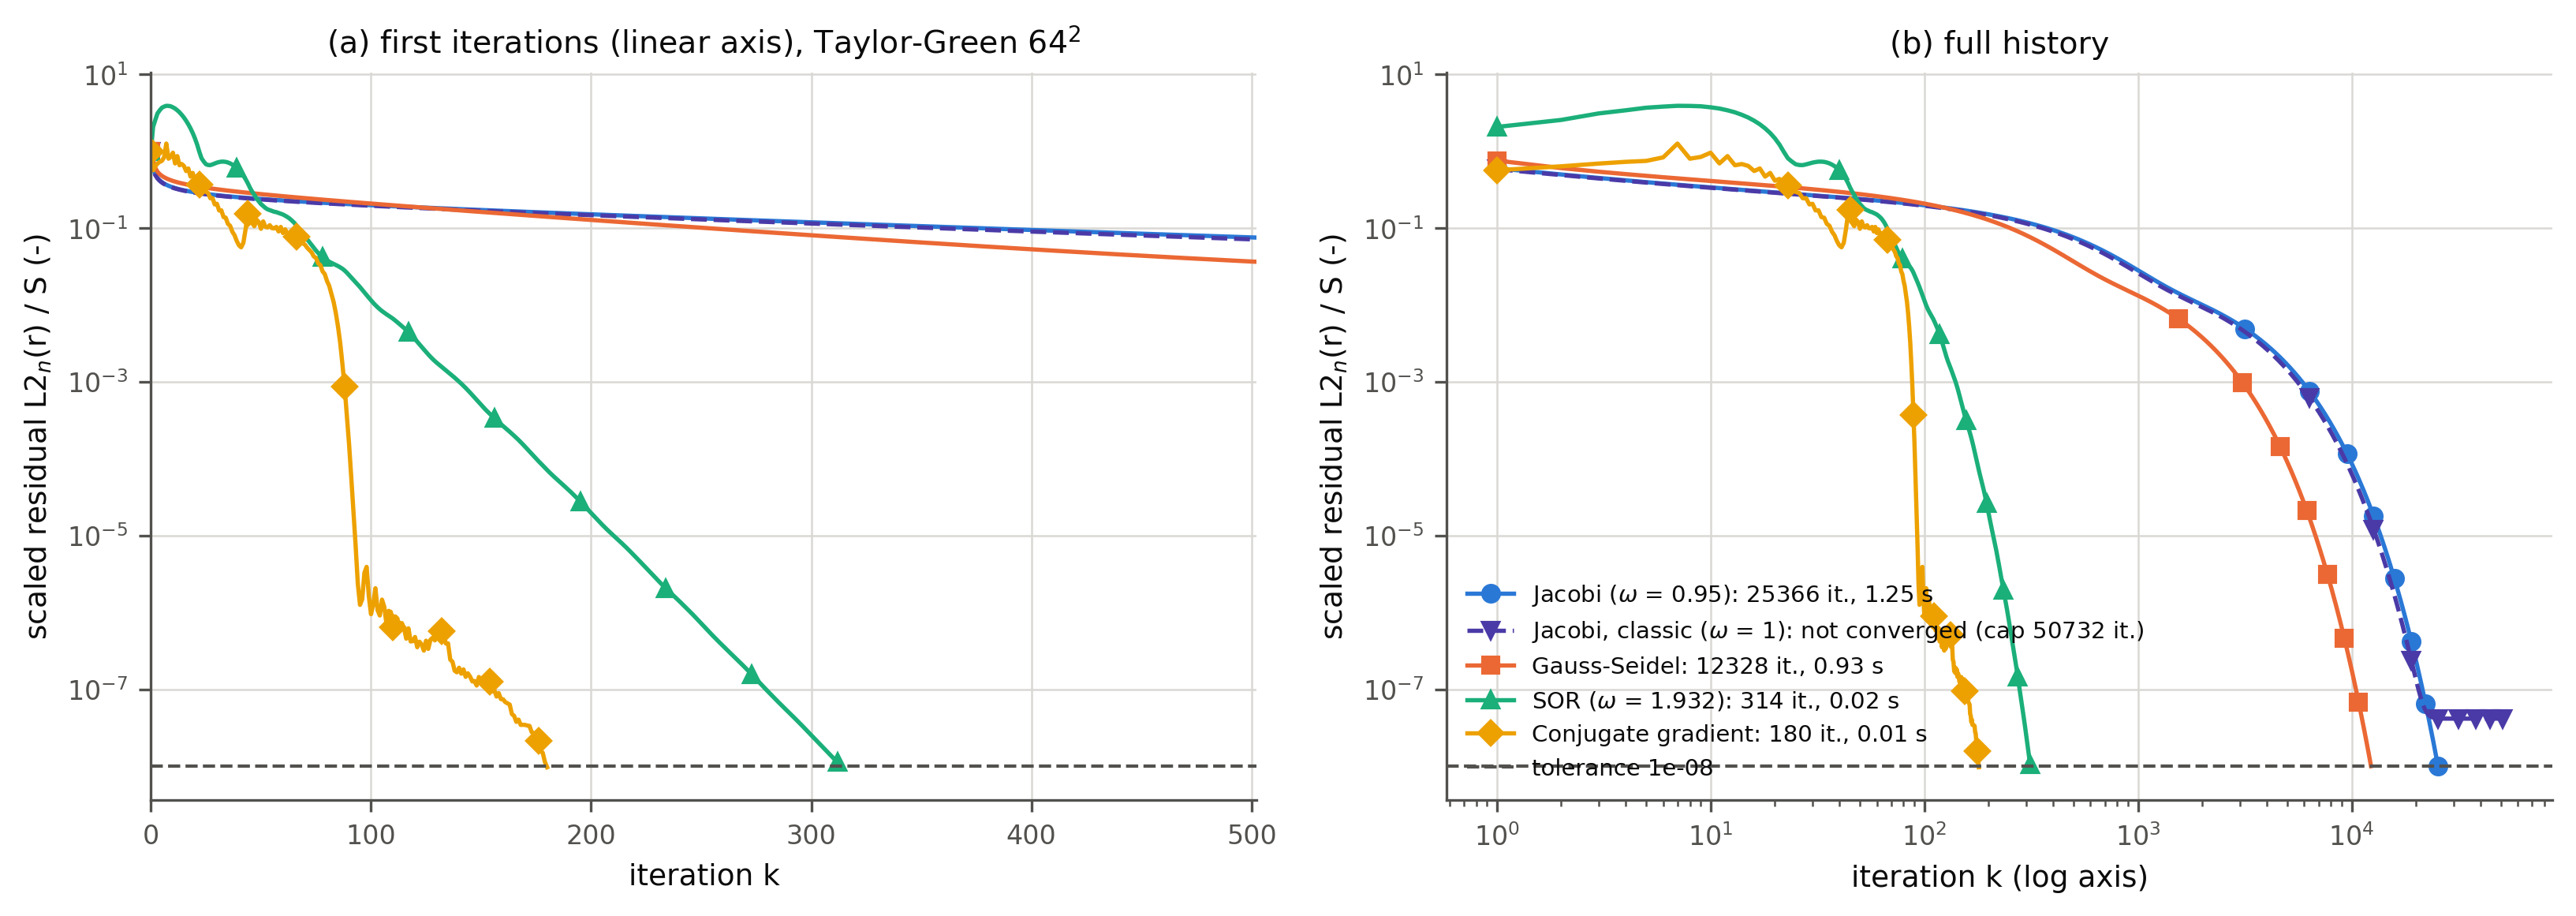
\includegraphics[width=\linewidth]{img/b_residuals.png}
\caption{Scaled residual history of five iterative solvers on the Taylor--Green $64^2$ Poisson system.}\end{figure}

\begin{table}[H]\centering\small
\begin{tabular}{@{}lrr@{}}\toprule
Solver ($64^2$, tol $10^{-8}$) & Iterations & Time\\\midrule
Jacobi ($\omega=0.95$) & 25\,366 & 1.3 s\\
Gauss--Seidel (red-black) & 12\,328 & 0.93 s\\
SOR ($\omega=1.932$) & 314 & 0.024 s\\
Conjugate gradient & 180 & 0.013 s\\
Jacobi, classic ($\omega=1$) & stalls at $4.2\times10^{-8}$ & --\\
Sparse direct (\code{spsolve}) & -- & $\approx$0.015 s\\\bottomrule
\end{tabular}\end{table}
Gauss--Seidel needs half the Jacobi iterations ($\rho_{GS}=\rho_J^2$); SOR and CG need 80--140$\times$ fewer. Classic Jacobi levels off above the tolerance: the checkerboard stall of Section~7.2. All solvers give the same pressure as the direct solve (agreement $<10^{-6}$).

\section{Iterations vs grid size and SOR stability}
\begin{figure}[H]\centering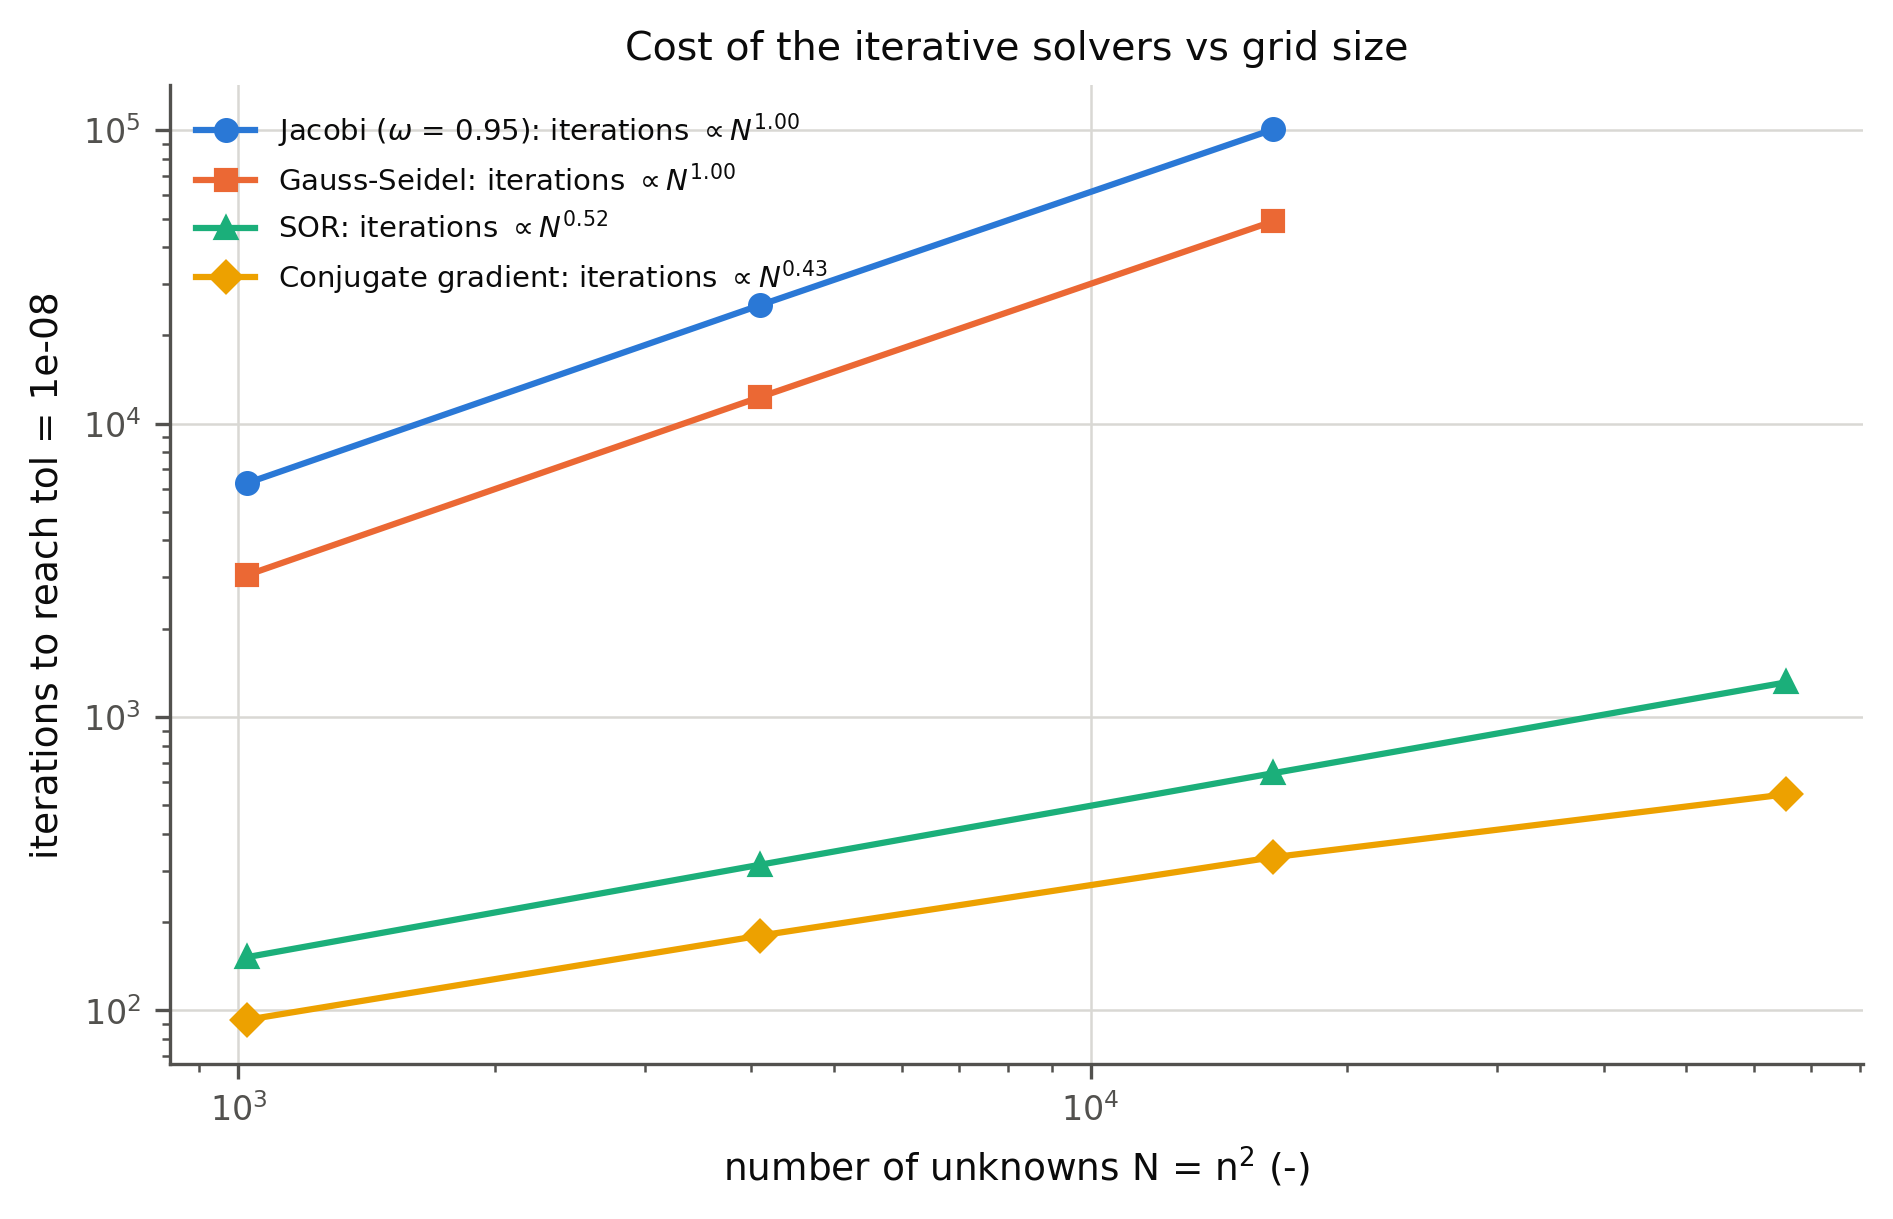
\includegraphics[width=0.7\linewidth]{img/fig14_iterations_vs_grid.png}
\caption{Iterations to converge vs number of unknowns $N$.}\end{figure}
Fitted exponents: Jacobi and Gauss--Seidel $N^{1.00}$, SOR $N^{0.52}$, CG $N^{0.43}$, as the theory predicts ($N$ for Jacobi/GS, $\sqrt N$ for optimal SOR and CG).

\begin{figure}[H]\centering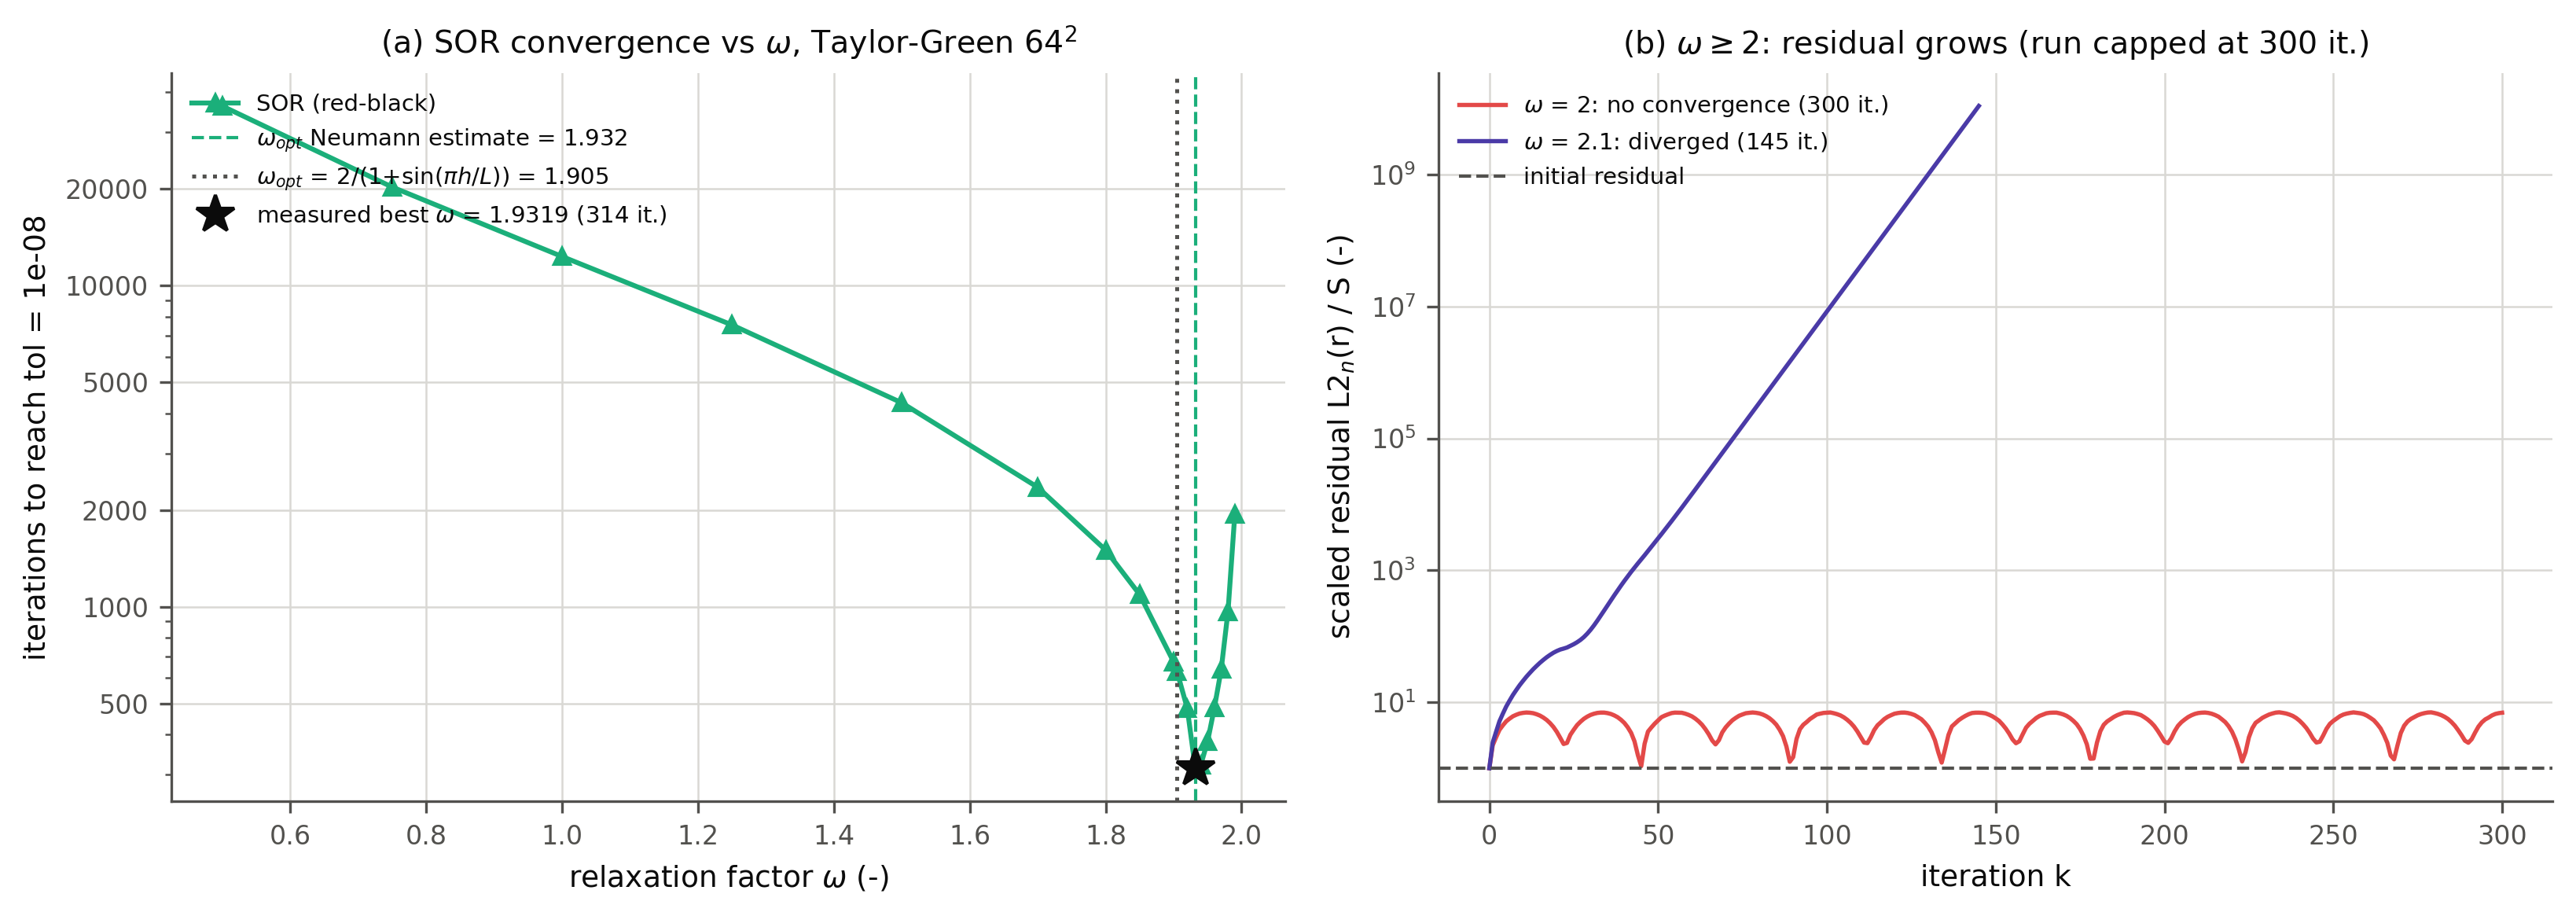
\includegraphics[width=\linewidth]{img/fig15_sor_stability.png}
\caption{(a) SOR iterations vs $\omega$; the measured optimum matches the Neumann estimate 1.932, not the Dirichlet formula 1.905. (b) $\omega=2$ does not converge and $\omega=2.1$ diverges (Kahan).}\end{figure}

\section{Residual vs change}
\begin{figure}[H]\centering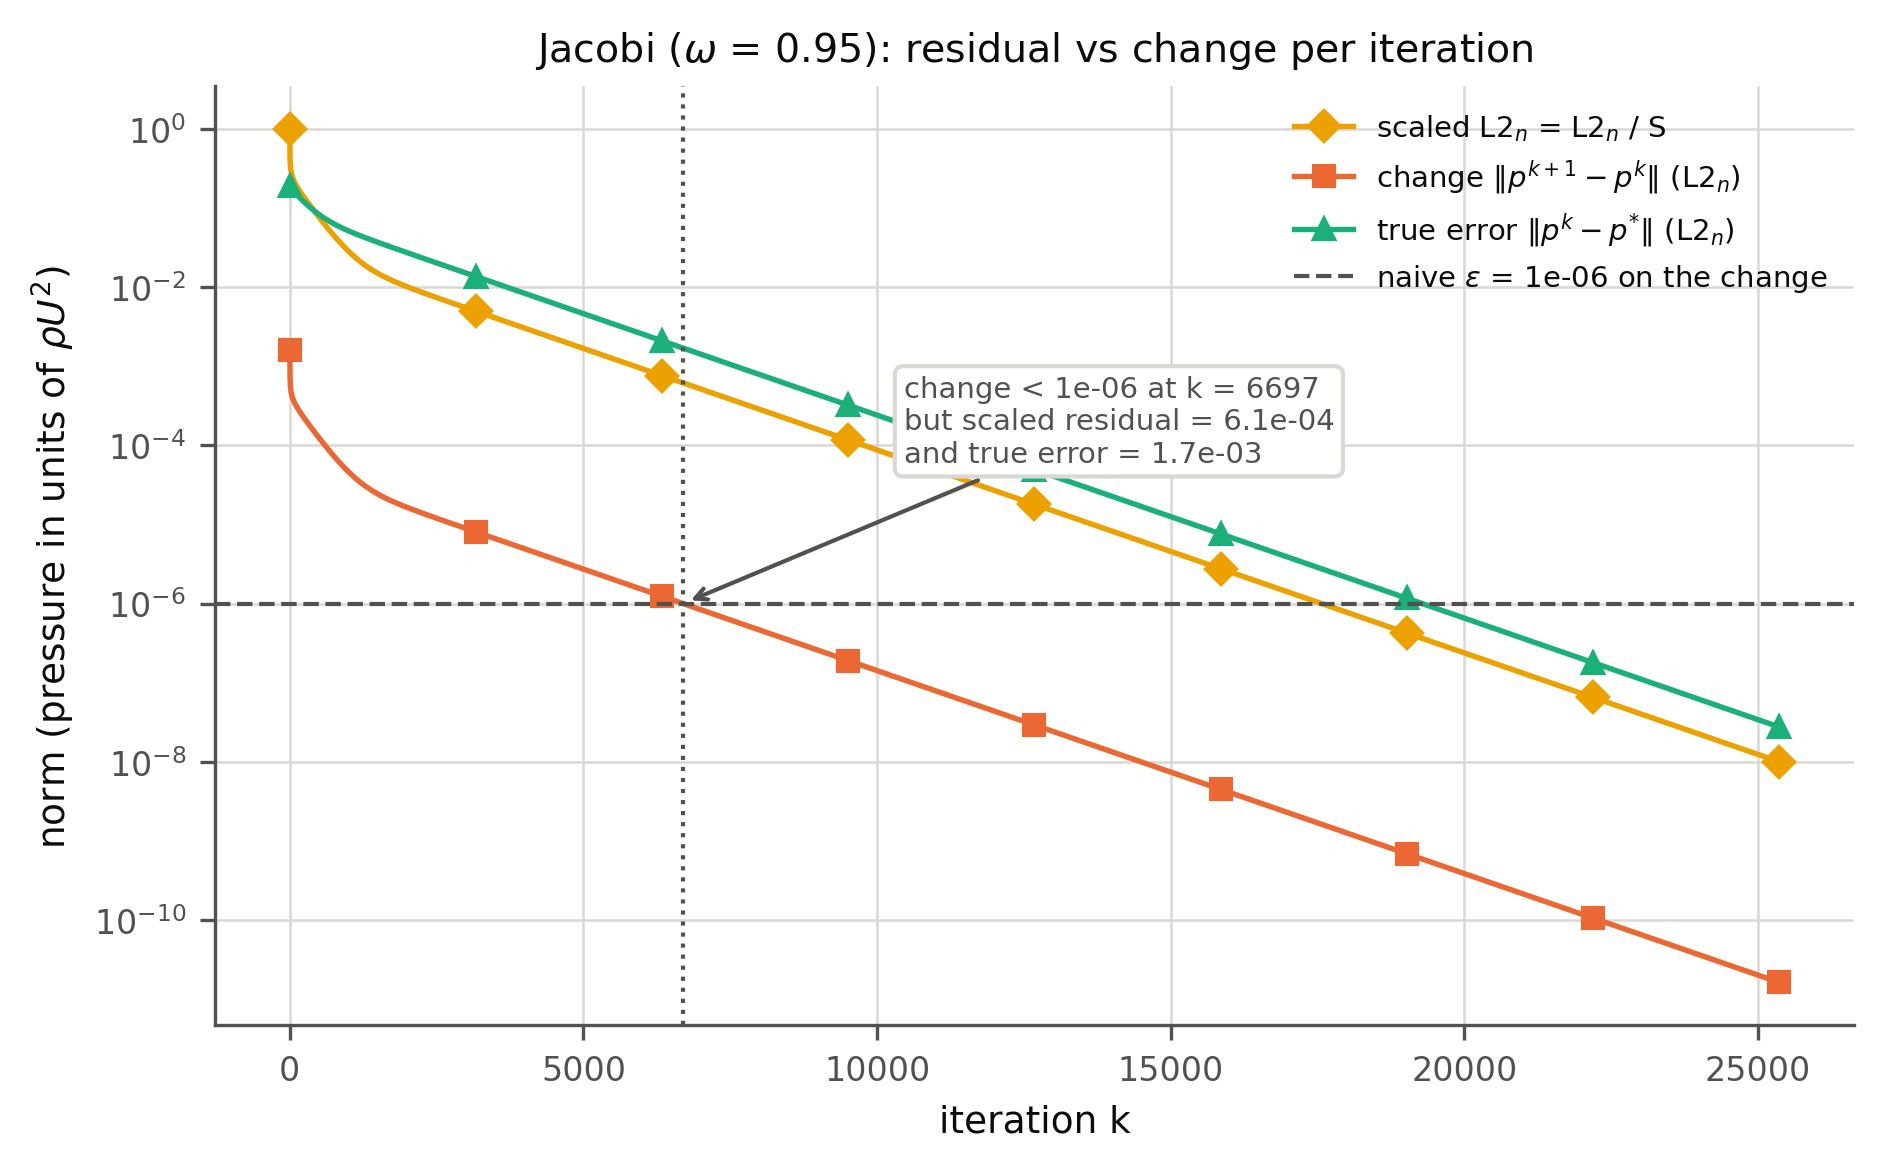
\includegraphics[width=0.72\linewidth]{img/fig13_residual_vs_change.png}
\caption{Jacobi: scaled residual, change per iteration and true error. When the change first drops below $10^{-6}$ the solution is still far from converged.}\end{figure}

\section{Norms across grids}
\begin{figure}[H]\centering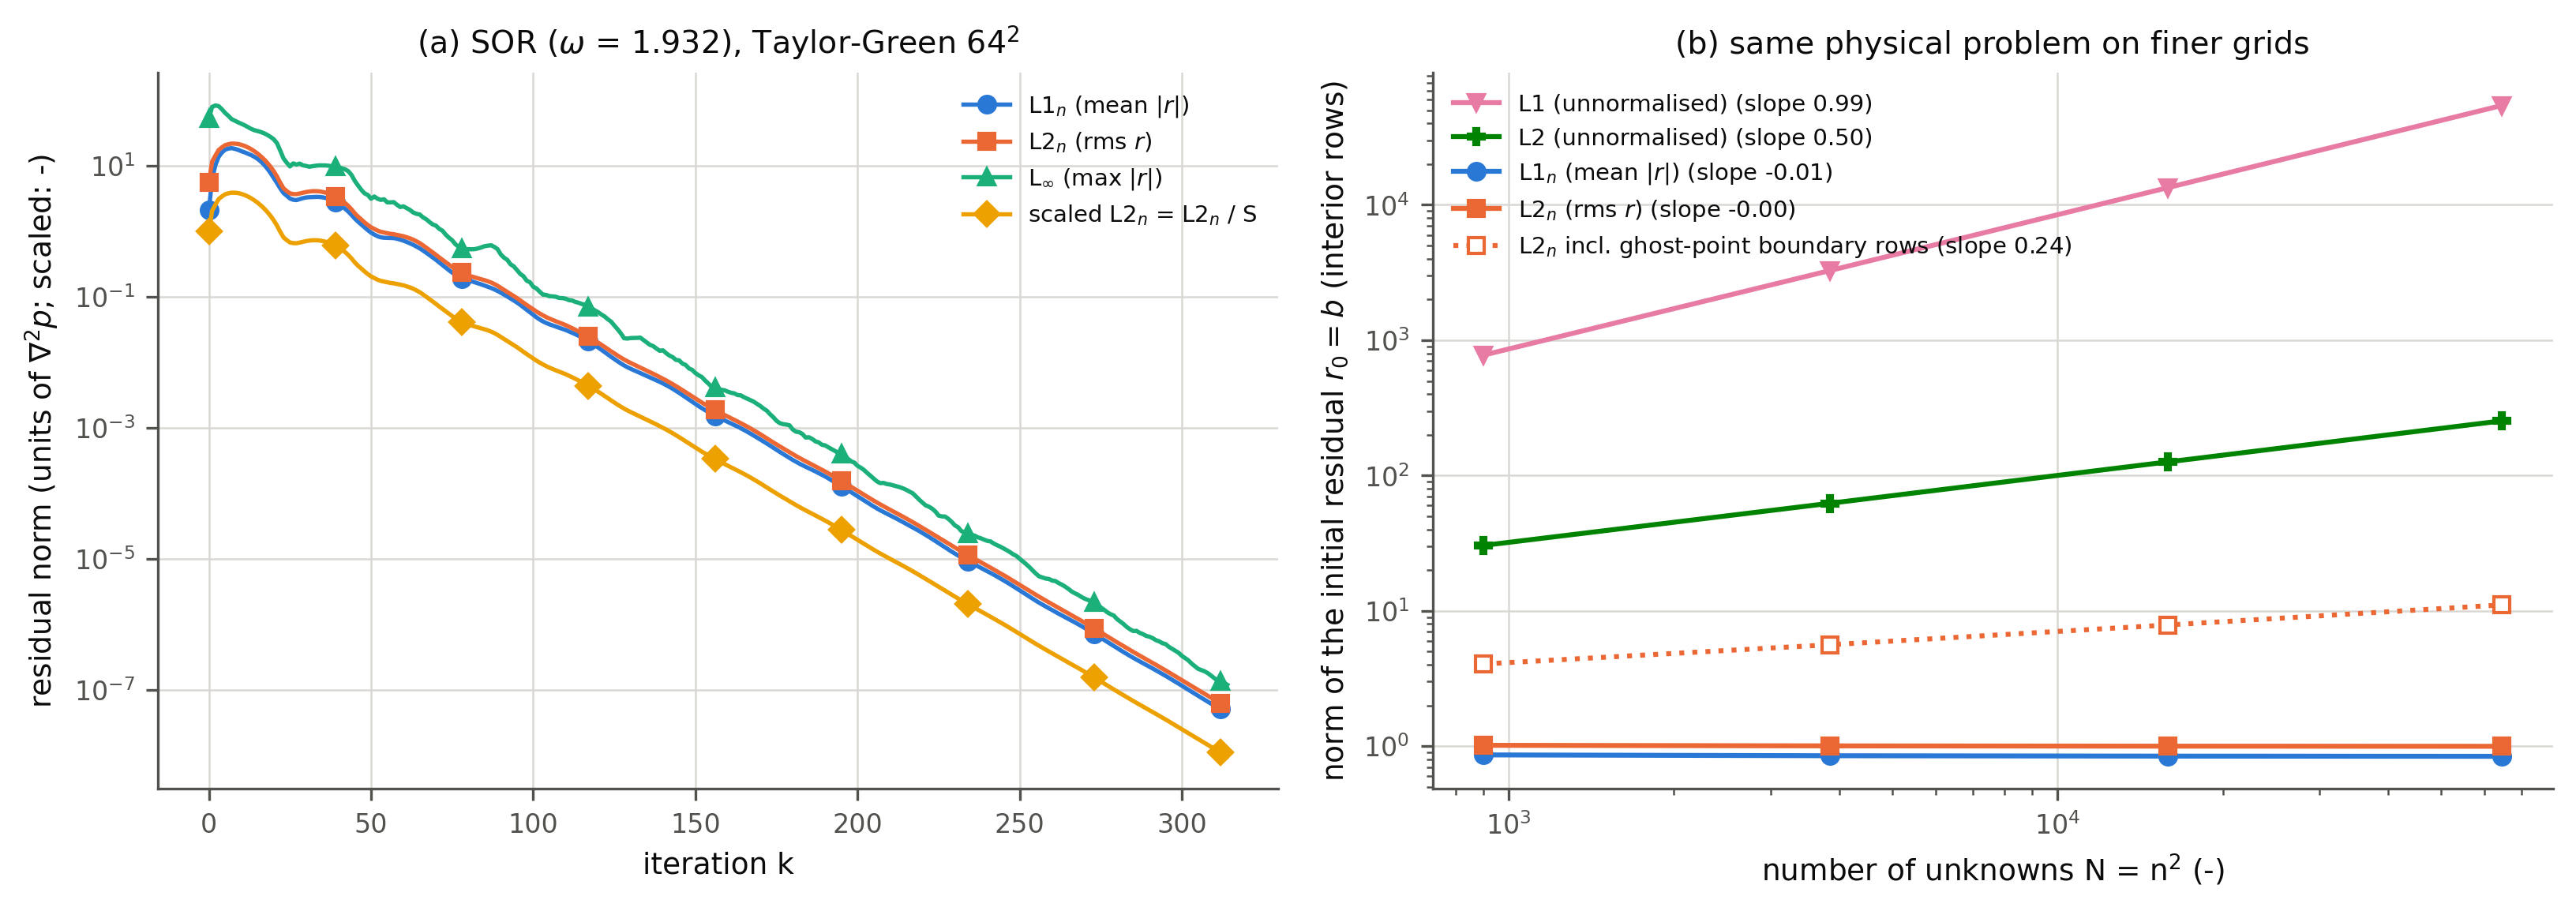
\includegraphics[width=\linewidth]{img/fig12_norm_comparison.png}
\caption{Different norms of the same residual. Unnormalised $L_1$, $L_2$ grow with grid size ($N^{0.99}$, $N^{0.50}$); normalised norms stay flat.}\end{figure}

\section{First- vs second-order schemes}
\begin{figure}[H]\centering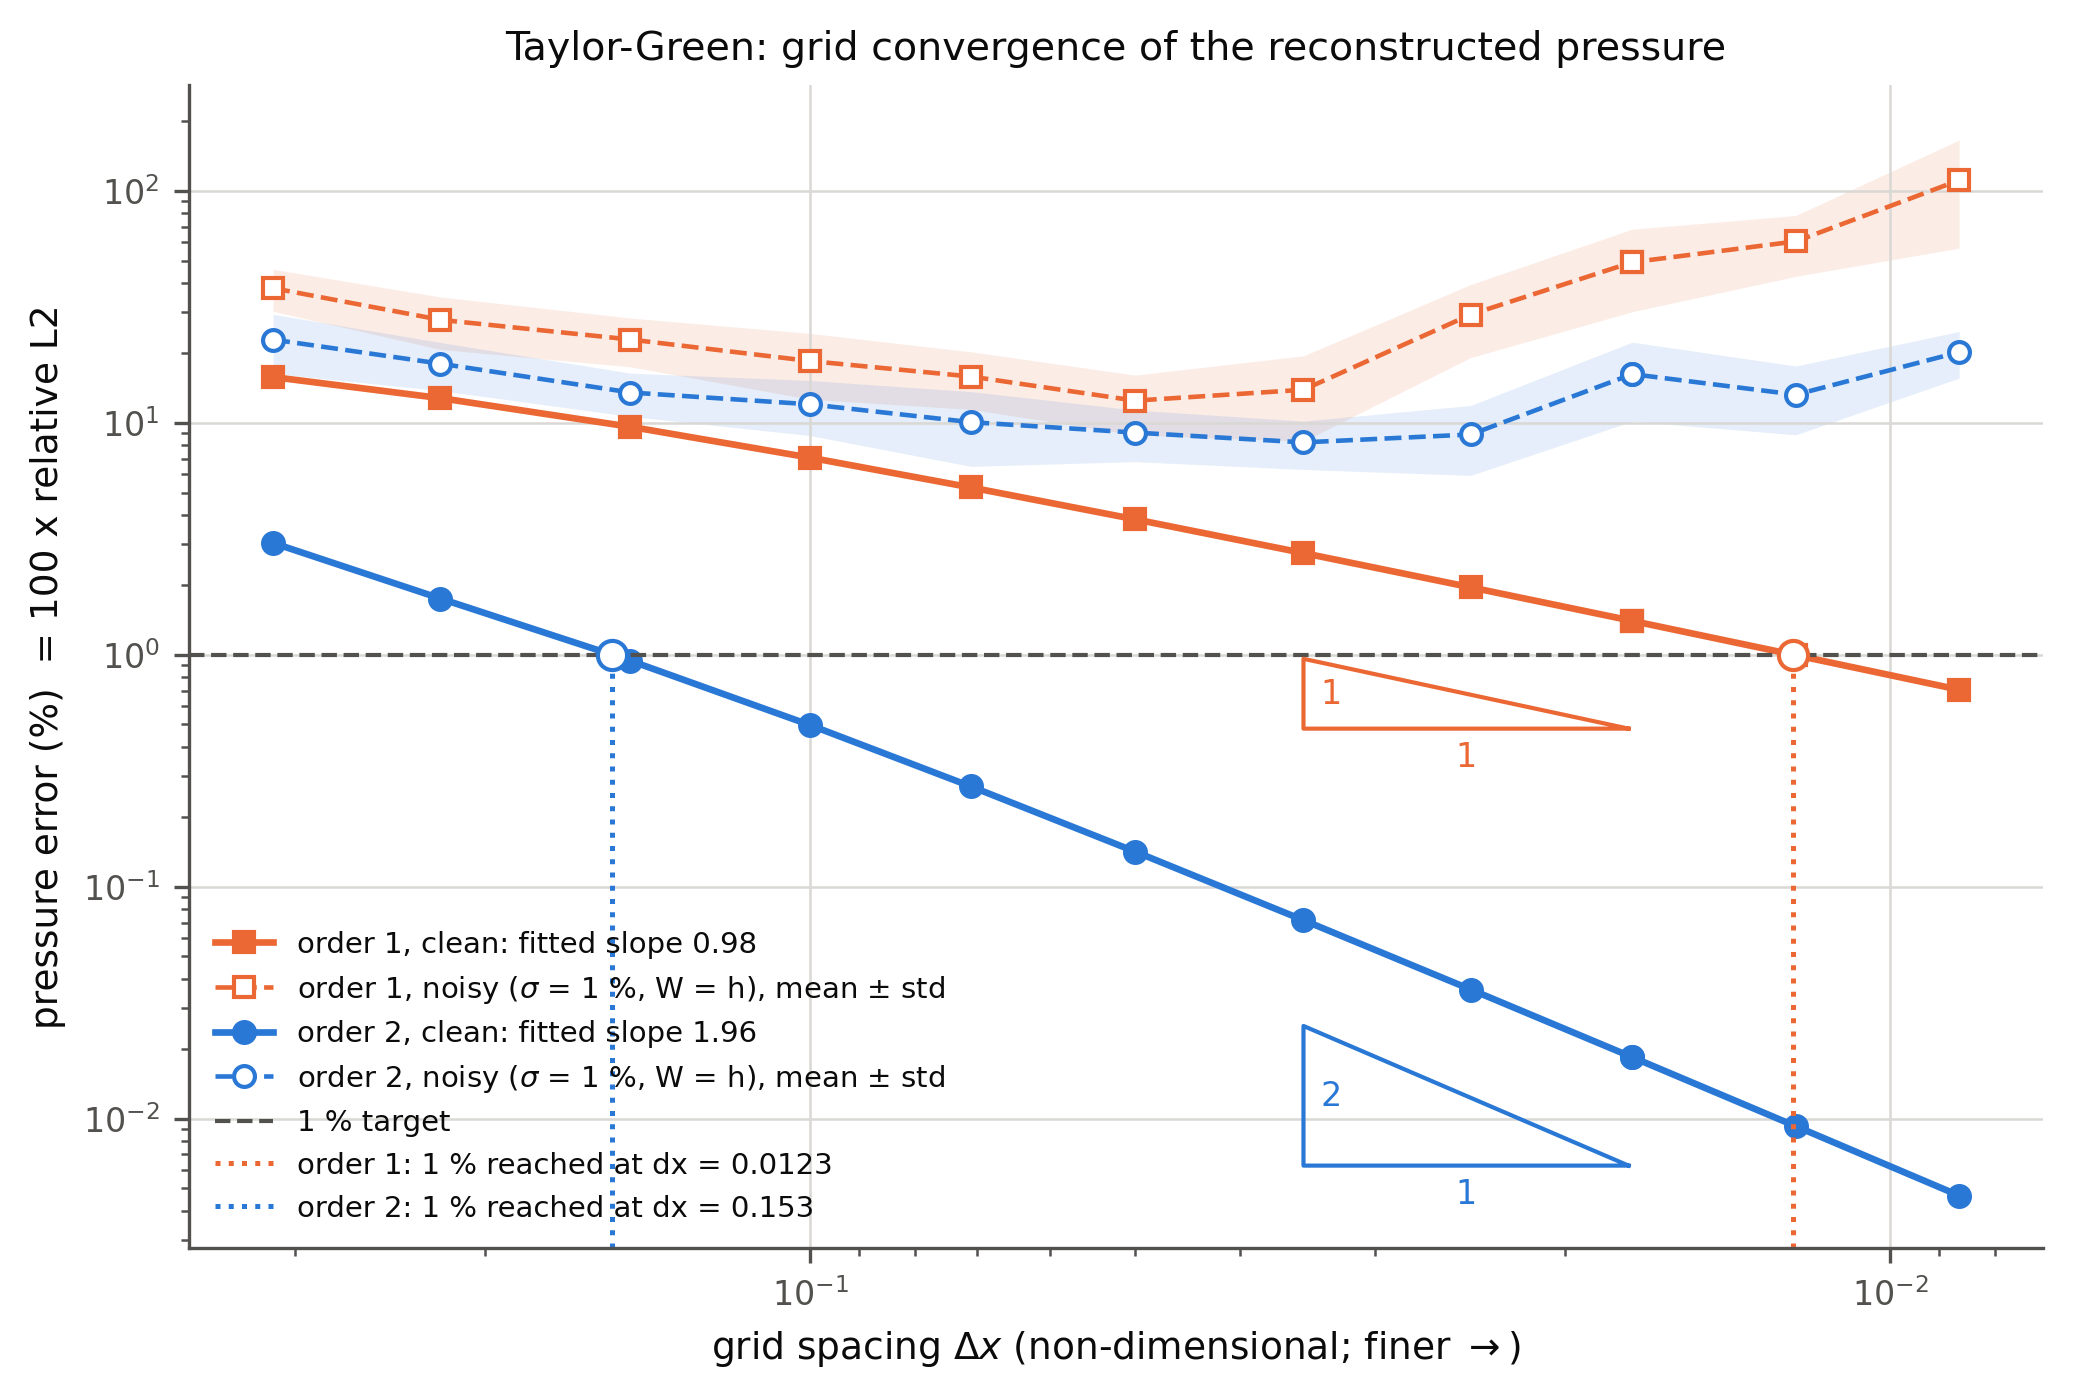
\includegraphics[width=0.72\linewidth]{img/b_order.png}
\caption{Grid convergence of the reconstructed pressure on Taylor--Green with first- and second-order stencils; dashed: 1\,\% noise.}\end{figure}

\begin{table}[H]\centering\small
\begin{tabular}{@{}lcccc@{}}\toprule
 & \multicolumn{2}{c}{Slope (finest 5 grids)} & \multicolumn{2}{c}{$\Delta x$ for 1\,\% error}\\
Case & order 1 & order 2 & order 1 & order 2\\\midrule
Taylor--Green & 0.98 & 1.96 & 0.0123 & 0.153\\
Kovasznay Re = 20 & 1.00 & 1.96 & 0.0033 (extrap.) & 0.026\\\bottomrule
\end{tabular}\end{table}
The second-order scheme reaches 1\,\% error on a grid about 12$\times$ coarser in each direction (Taylor--Green). To halve the error, order 1 must refine $\Delta x$ by 2, order 2 only by $\sqrt2$. With 1\,\% noise both curves level off and rise again; the second-order scheme stays lower.

\textbf{Why order 1 gives slope 1 even with an $O(1)$ boundary error.} The first-order Neumann row has an $O(1)$ local truncation error, but it acts only on a layer of width $O(h)$, so the global error is $O(h)$, the same argument that makes the second-order scheme's $O(h)$ boundary rows globally $O(h^2)$.
